\documentclass[article]{jss}

%% -- LaTeX packages and custom commands ---------------------------------------

%% recommended packages
\usepackage{thumbpdf,lmodern}

%% another package
\usepackage{framed}
\usepackage{dsfont}
\usepackage{amsmath,amsthm}
\usepackage{amsfonts}
\usepackage{amssymb}
\usepackage{rotating}
\usepackage{orcidlink}
\usepackage{enumerate}
\usepackage{float} % to allow H for figure position
\usepackage{longtable}
\usepackage[tableposition=below]{caption}
\captionsetup[longtable]{skip=0.9em}
\usepackage{subcaption}
\usepackage{cleveref}
\usepackage{todonotes}
\usepackage{enumitem}
\usepackage{comment}


% track changes
\usepackage[]{changes}

%Algorithm
\usepackage{algorithm}
\usepackage{algorithmic}

%% new custom commands
\newcommand{\class}[1]{`\code{#1}'}
\newcommand{\fct}[1]{\code{#1()}}
\theoremstyle{definition}
\newtheorem{definition}{Definition}

\input{notation.tex}


%% -- Article meta-information (author, title, ...) -----------------------------

%% - \author{} with primary affiliation
%% - \Plainauthor{} without affiliations
%% - Separate authors by \And or \AND (in \author) or by comma (in \Plainauthor).
%% - \AND starts a new line, \And does not.
%\author{Sebastian Fischer \And Lukas Burk \And Florian Pfisterer \And Carson Zhang \AND Bernd Bischl \And Martin Binder}
\author{Sebastian Fischer~\orcidlink{0000-0002-9609-3197} \\
    LMU Munich \\
    MCML \\
    \And Lukas Burk~\orcidlink{0000-0001-7528-3795} \\
    LMU Munich, MCML \\
    Leibniz Institute for\\Prevention Research and\\Epidemiology - BIPS \\
    University of Bremen
    \AND Carson Zhang \\
    LMU Munich \\
    \And Bernd Bischl~\orcidlink{0000-0001-6002-6980} \\
    LMU Munich \\
    MCML \\
    \And Martin Binder~\orcidlink{0009-0008-2578-2869} \\
    LMU Munich \\
    MCML \\
}

\Plainauthor{Sebastian Fischer, Lukas Burk, Florian Pfisterer, Carson Zhang, Bernd Bischl, Martin Binder}

%% - \title{} in title case
%% - \Plaintitle{} without LaTeX markup (if any)
%% - \Shorttitle{} with LaTeX markup (if any), used as running title
\title{\mlrttorch{}: A Deep Learning Framework in \rlang{} based on \mlrt{} and \torch{}}
\Plaintitle{mlr3torch: A Deep Learning Framework in R based on mlr3 and torch}


%% - \Abstract{} almost as usual
\Abstract{
    Deep learning (DL) has become a fundamental approach in modern machine learning (ML) with applications across various domains.
    We introduce the \rlang{} package \pkg{mlr3torch}, a comprehensive and extensible DL framework that seamlessly integrates into the \pkg{mlr3} ecosystem.
    Built on the \pkg{torch} package, \pkg{mlr3torch} simplifies the creation, training, and evaluation of neural networks for both tabular data and generic tensors (e.g., images) for classification and regression.
    The package comes with predefined architectures, and \torch{} models can easily be converted into \mlrt{} learners. It also allows users to define neural networks as graphs.
    This representation is based on the graph language defined in the \pkg{mlr3pipelines} \rlang{} package and allows users to define the entire DL workflow, including preprocessing, data augmentation, and network architecture, in a single graph.
    Being fully integrated into the \pkg{mlr3} ecosystem, the package allows for standardized resampling, benchmarking, preprocessing, and more.
    We explain the package's basic functionality and show how to customize or extend it to new domains.
    Furthermore, we demonstrate the package's capabilities through applications such as hyperparameter tuning, fine-tuning of pre-trained models, and defining architectures for multimodal data.
    Finally, we present some runtime benchmarks.
}

%% - \Keywords{} with LaTeX markup, at least one required
%% - \Plainkeywords{} without LaTeX markup (if necessary)
%% - Should be comma-separated and in sentence case.
\Keywords{deep learning, machine learning, \rlang{}}
\Plainkeywords{deep learning, machine learning, R}

%% - \Address{} of at least one author
%% - May contain multiple affiliations for each author
%%   (in extra lines, separated by \emph{and\$.
%% - May contain multiple authors for the same affiliation
%%   (in the same first line, separated by comma).
\Address{
  Sebastian Fischer \\
  Insitut f\"ur Statistik \\ Ludwig-Maximilians-Universit\"at M\"unchen, Germany \\
  Ludwigstr. 33, 80539 Munich, Germany \\
  Munich Center for Machine Learning (MCML), Germany \\
  E-mail: \email{sebastian.fischer@stat.uni-muenchen.de}
}


\begin{document}

\begin{comment}

Done:
\begin{itemize}
  \item [x] Ensure consistent <- over =
  \item [x] max 30 pages (not a strict requirement). We are sightly above this limit, so should be fine
  \item [x] use \top instead of $^T$
  \item [x] For referring to subsections, do not use Subsection x.y, just Section x.y.
  \item [x] All captions should appear below the corresponding figure/table.
  \item [x] Abkürzungen konsistent verwenden: DL, ML, NLP etc.
  \item [x] Use \code{...} instead of \texttt{...} for inline code
  \item [x] Cite all datasets
  \item [x] use proglang everywhere
      * [x] Rust
      * [x] Go
      * [x] Python
      * [x] R
      * [x] C++
      * [x] Julia
  \item [ ] use pkg everywhere
      * [x] " mlr3"
      * [x] " torch "
  \item [x] never use (\cite{...}). (use \citep{} for that)
  \item [x] \title in title style
  \item [x] Do not use additional formatting for specific words unless explicitly required by the JSS style guide, e.g., --> remove emph and textit etc.
  \item [x] No comments in Code, this information should be presented in the normal latex text
  \item [x] In order to use markup in section headers, you can use: \section[Calling C++ from R]{Calling \proglang{C++} from \rlang{}}
  \item [x] To refer to equations, one can use either Equation~\ref{...} (with capitalization) or (\ref{...}) with the former being preferred if the number of equation references is not too large.
  \item [x] The captions should be in sentence style and end with a period. No additional formatting (such as \emph, \bf or \it) should be used for the caption.
  \item [x] All table row/column headers should also be in sentence style. There should not be further footnote-style annotations in tables; these should all be placed in the caption.
  \item [x] For bullet lists/itemized lists please use either a comma, semi-colon, or period at the end of each item
  \item [x] annotations of figures/tables (including captions) in sentence style
  \item [x] Add comma after e.g., and i.e., to prevent latex from interpreting as end of sentence
  \item [x] Abbreviations should be spelled in upper-case letters without additional formatting (i.e., without periods, without small caps, italics, etc.). All abbreviations should be introduced with their expansion where the expansion should not be capitalized. (Exceptions are, of course, when the expansion contains proper names or the first word is the first word of a sentence.) Examples would include:
  \item [x] \section, \subsection, etc. in sentence style (in sentence style, only first word of sentence and forst word after - or : is capitalized)
  \item [x] Text in figures: In particular, this means that annotations should not be too large or too small. As a rough guidance, graphics annotation should be a about the size of the figure caption or a little bit smaller.
    \item [x] Figures, tables and equations are marked with a \label and referred to by \ref, e.g., Figure~\ref{...} Software packes are \cite{}d properly.
    \item [x] CodeInput and CodeOutput used correctly everywhere?
    \item [x] For R packages that don't have an official citation, use citation("foo"), but make sure that \proglang{} and \pkg{} are used correctly
\end{itemize}

References:
\begin{itemize}
    \item [x] Use \proglang{} and \pkg{} also there
    \item [x] all titles in the BibTeX file in title style.
    \item [x] For books with an edition, this should be indicated as 2nd, 3rd, etc.
    \item [x] If software does not say provide way for citation, use  the following:
    \@Manual{SAS-STAT,
        author  = {{\proglang{SAS} Institute Inc.}},
        title   = {\proglang{SAS/STAT} Software, Version~9.1},
        year    = {2003},
        address = {Cary, NC},
        url     = {https://www.sas.com/}
    }
\end{itemize}

Code:

\begin{itemize}
    \item [ ] Run code one more time and copy results to script
    \item [ ] We need to provide a simplified version of the script reproducing the results that can run on a regular PC. (https://www.jstatsoft.org/authors#manuscript-preparation) -> maybe I can just run this on GitHub actions CI?
    \item [ ] to facilitate review, authors are strongly encouraged to provide an output file that shows the results from running the single standalone replication script so that this can be compared against the results presented in the manuscript. For R submissions, this should be done by providing a file "code.html" created by running knitr::spin("code.R") on the replication script "code.R" which should include a call to sessionInfo() at the end.
    \item [ ] Check that networks / learners that are not trained here still can be trained and are correctly constructed
    \item [ ] Check that we are citing the correct R packages for those packages without a paper (sessionINfo))
    \item [ ] Run code at the end twice for reproducibility
    \item [x] sessionInfo in code
    \item [x] ensure that caching is enabled in code because otherwise temp directory might be deleted for the melanoma dataset on linux
\end{itemize}

\begin{itemize}
    \item 1. [ ] one more grammarly
    \item 2. [ ] one more read (also focus on citation display and go through citations at the end
    \item 3. [ ] manuscript can be compiled using pdflatex
    \item 4. [ ] Nothing goes beyond left and right margin
\end{itemize}

Final submission:

\begin{itemize}
    \item [ ] Correct mlr3torch version
    \item [ ] release jss branch in mlr3torch as submission
    \item [ ] Size limit: Upload not more than 50 MB
    \item [ ] submission must contain: pdf manuscript, source code, replication materials
    \item [ ] Source code must be submitted in ASCII files
\end{itemize}


\end{comment}

%\input{1-introduction}
%\input{2-building-blocks}
%\input{3-extending}
%\input{4-use-cases}
%\input{5-runtime-evaluation}

\section{Introduction and related work}

Deep learning (DL) has had a profound influence on various fields, including computer vision, audio, and natural language processing.
More recently, there has also been an increased focus on applying DL to tabular data \citep{ref-borisov2022deep}.
Training deep neural networks requires software that supports hardware-accelerated tensor operations and automatic differentiation.
Together, these two components enable the definition and training of neural network architectures using gradient-based optimization.
However, these libraries can be employed for more than just training deep neural networks. For instance, they can be used for Gaussian processes, as in the \pkg{GPyTorch} package \citep{gardner2018gpytorch}.

The dominant programming language for DL is \python{} \citep{ref-van1995python}, for which the libraries \tensorflow{} \citep{ref-abadi2016tensorflow}, \pytorch{} \citep{ref-pytorch}, and \pkg{JAX} \citep{ref-jax2018github} are primarily developed.
Historically, \tensorflow{} popularized static computation graphs, enabling optimized deployment. Meanwhile, \pytorch{} gained traction due to its dynamic graph approach, prioritizing flexibility and allowing for easier debugging.
Nowadays, \tensorflow{} also supports eager execution, while \pytorch{} also allows for static compilation, making it apparent that both approaches have their merit.
Still, due to its flexibility and ease of use, \pytorch{} is arguably the de-facto standard for DL research, but \tensorflow{} and \pkg{keras} are still relatively common in production stacks.
More recently, \pkg{JAX} introduced a functional approach that can be described as \pkg{NumPy} \citep{ref-harris2020array}, enhanced with hardware acceleration and automatic differentiation.
Another noteworthy \python{} library is \pkg{tinygrad} \citep{ref-tinygrad}, which strives to be a minimal, lightweight DL framework designed for simplicity and easy extensibility across multiple hardware platforms.

These libraries focus primarily on the core building blocks of DL, leaving higher-level abstractions, such as training loops, model management, preprocessing, data augmentation, and experiment tracking, to other frameworks.
One example of such a framework is \pkg{Keras} \citep{ref-chollet2018keras}, which offers a high-level API that is both integrated into \tensorflow{} but also available as a standalone multi-backend library with support for \pytorch{}, \tensorflow{}, and \pkg{JAX}. Furthermore, \pkg{PyTorch Lightning} \citep{ref-lightning2019} and \pkg{fastai} provide higher-level DL toolboxes exclusively for \pytorch{}, and \pkg{Flax} \citep{ref-flax} offers similar capabilities for \pkg{JAX}.

Languages other than \python{} also have DL libraries of their own.
These include \julia{} \citep{ref-bezanson2017julia}, which offers a full DL stack via \flux{} \citep{ref-innes2018flux}, \rust{} \citep{ref-matsakis2014rust} with its crates \pkg{Burn} \citep{ref-burn} and \pkg{Candle} \citep{ref-candle}, and \proglang{Go} \citep{ref-go} with \pkg{gomlx} \citep{ref-gomlx}.
In \cpp{} there is \pkg{LibTorch}, the \cpp{} backend for \pytorch{}, which can also be used as a stand-alone \cpp{} library.

In the \rlang{} language \citep{ref-R-base}, many DL packages are available, but modern practice has consolidated on a few highly expressive, modular frameworks with corresponding counterparts in the \python{} ecosystem.
One of these is  \pkg{torch} \citep{ref-torch2025}, which is a native DL framework that is built directly on top of \pkg{LibTorch} and works similarly to \pytorch{}.
Various extensions exist for \torch{}.
For example, the \pkg{torchvision} package is a collection of pre-trained models, datasets, and preprocessing operations for computer vision tasks \citep{ref-r-torchvision}.
Furthermore, \pkg{luz} \citep{ref-luz2023} and \pkg{cito} \citep{ref-cito2024} are two higher-level DL frameworks for \rlang{} built on top of \torch{}.

Other backends are supported via \pkg{keras3} \citep{ref-keras32025} and \pkg{tensorflow} \citep{ref-r-tensorflow2024}, which both wrap the corresponding \python{} libraries via \pkg{reticulate} \citep{ref-reticulate2025}, as is the case for \pkg{fastai} \citep{ref-fastai}.
The main advantage of \pkg{torch} over these reticulate wrappers is that it does not have the \python{} dependency, allows for easier debugging, and requires less marshaling for the communication of objects between \rlang{} and \python{}.
A disadvantage is the higher development cost.

Besides these general-purpose DL frameworks, more specialized libraries exist, focusing on selected architectures or training procedures.
This includes the packages \pkg{nnet}, \pkg{neuralnet}, \pkg{deepnet}, \pkg{RSNNS} \citep{ref-nnet, ref-neuralnet, ref-deepnet, ref-rsnns}.
While these packages are a good place to start, they do not offer GPU acceleration and are rather limited with respect to their expressiveness.
While \pkg{h2o} does allow for GPU training, it is similarly restricted with respect to the available architectures \citep{ref-h2o}.

In addition to specialized DL toolkits, there are other, more general-purpose ML libraries that primarily focus on tabular data.
In \python, there is \sklearn{} \citep{ref-pedregosa2011scikit-learn}, in \julia{} there is \mlj{} \citep{ref-blaom2020mlj}, and \rlang{} has \tidymodels{} \citep{ref-kuhn2020tidymodels} and \pkg{mlr3} \citep{ref-mlr32019} with their respective predecessors \pkg{caret} \citep{ref-kuhn2021caret} and \pkg{mlr} \citep{ref-bischl2016mlr}, both of which are still widely used.
From the perspective of these general ML frameworks, neural networks are just one type of learning method, alongside other approaches, such as statistical models, support vector machines, and tree-based systems.
Connector packages exist to connect DL methods to these generic APIs.
For example, the \pkg{skorch} package \citep{ref-skorch} for integrating \pytorch{} into \sklearn{}, \pkg{MLJflux} \citep{ref-MLJFlux} for \flux{} and \mlj{}, and \pkg{brulee} \citep{ref-brulee2025} for \torch{} and \tidymodels{}.

The core idea of \mlrttorch{} is to extend the \mlrt{} ecosystem with comprehensive DL capabilities tailored to its user base.
For example, other ML models can be seamlessly replaced by DL approaches, and out-of-memory data can be preprocessed in a manner analogous to the standard preprocessing of tabular data in \mlrt{}.
Through this integration, \mlrttorch{} inherits the full range of \mlrt{}’s features — such as preprocessing, benchmarking, and hyperparameter tuning \citep{ref-mlr3tuning2024} — which represents one of its key advantages.
In addition, \mlrttorch{} provides high-level infrastructure, including training and evaluation loops, that substantially simplify the training of neural networks compared to directly using \pkg{torch} or \pkg{tensorflow}.
Although \pkg{cito} offers similar functionality, it is built around a much simpler and thus less expressive interface, resembling the specialized libraries discussed above, but using \pkg{torch} as a backend.
The comparison with \pkg{brulee} is similar, as the package only supports relatively simple architectures like MLPs.
\pkg{luz}, by contrast, is currently more flexible than \mlrttorch{}, and can, for example, be used to train variational autoencoders, whereas \mlrttorch{} is currently restricted to regression and classification.
However, in cases where \mlrttorch{} is applicable, it offers a richer feature set, including predefined tabular architectures or more evaluation measures.
The package most closely related in spirit to \mlrttorch{} is \pkg{keras3}, which wraps the corresponding \python{} library and provides a more mature, feature-complete framework than \mlrttorch{} and its \torch{} backend.
For example, it also supports text processing, for which there is currently no proper support in \mlrttorch{}.
Nevertheless, the reliance on \python{} introduces the disadvantages discussed earlier, including more challenging debugging.
Moreover, \mlrttorch{} distinguishes itself from \pkg{keras3} by offering a unified graph language for expressing ML workflows that extend beyond neural networks, enabling, for example, straightforward integration of DL models with other ML models via stacking \citep{ref-mlr3book-chap8}.
The comparison to \pkg{fastai} is similar: as a \python{} wrapper, it inherits the strengths and limitations of building on a mature \python{} library.
Both of these packages also do not offer the extensive hyperparameter tuning capabilities available for \mlrttorch{}.

\paragraph{Contributions} The \pkg{mlr3torch} package adds extensive DL capabilities to the \mlrt{} machine learning (ML) framework, which is a collection of \rlang{} packages that provide a unified interface to ML in \rlang{}.
Currently, it supports working with tabular data and generic tensors for supervised classification and regression.
Neural network architectures can be defined with different levels of customizability.
First, there are predefined architectures, such as vision learners from the \pkg{torchvision} \rlang{} package \citep{ref-r-torchvision}, or tabular architectures \citep{gorishniy2021revisiting}.
For full control, it is possible to define custom neural network modules in \rlang{} \torch{} and easily convert them to \mlrt{} \code{Learner}s.
Furthermore, \mlrttorch{} allows one to represent neural network architectures using the graph language defined in \mlrtpipelines{}, thereby making it possible to represent the entire modeling workflow, including preprocessing and data augmentation, as well as the neural network architecture, in a single workflow description, similar to how it is possible in \keras{} \citep{ref-chollet2018keras}.
Finally, the package is designed with extensibility in mind. The training loop is customizable via a callback mechanism, and it is easy to inherit from predefined classes for full control.

In the following sections, we provide an overview of the package. First, we give a brief overview of DL and the main \rlang{} packages \mlrttorch{} builds upon, as discussed in~\Cref{sec:background}.
Next, \Cref{sec:building-blocks} will summarize the package's main building blocks, including the data representation, the learner class, and neural network graph representation.
\Cref{sec:extending} will show how to extend the package. This is followed by some practical use cases in \Cref{sec:use-cases}.
There, we will cover hyperparameter tuning, fine-tuning, and constructing neural networks for multimodal problems.
To provide insight into the package's runtime performance, we will present benchmarks in~\Cref{sec:benchmarks}.
Finally, we will summarize the package and future directions in \Cref{sec:conclusion}.

\section{Background}\label{sec:background}


\subsection{Deep learning}\label{sec:background_dl}
% Other JSS publications also have this. This should be relatively short.
% I think maybe we should also include a section on the history of DL, i.e., how it came to be, who did what, etc.

Deep learning is an area of machine learning that uses neural networks to model complex patterns in data.
In recent years, neural networks have had a significant impact on fields such as computer vision, text generation, and speech recognition.
The simplest architecture is the multi-layer perceptron (MLP), which combines (affine-)linear transformations with nonlinear activation functions:

\begin{align}
f_{\boldsymbol{\theta}}(\mathbf{x}) &=
  \phi_{L}\!\bigl(
    W_{L}\,\phi_{L-1}\!\bigl(
      W_{L-1}\,\dotsm\phi_{1}(W_{1}\mathbf{x}+b_{1}) \ldots )+ b_{L - 1}
    \bigr)+b_{L}
  \bigr),
\end{align}

\noindent
with \(W_{\ell}\in\mathbb{R}^{d_{\ell}\times d_{\ell-1}}\), \(b_{\ell}\in\mathbb{R}^{d_{\ell}}\) and \(\theta = \{W_1, \ldots, W_L, b_1, \ldots, b_L\}\) for \(\ell=1,\dots,L\).

In general, almost all neural network architectures can be represented as directed acyclic graphs (DAGs).
Each node in the graph represents a possible parametrized, differentiable transformation that takes in one or more tensors as input and outputs one or more tensors.
Edges go from layer outputs to layer inputs, defining the data flow between operations.

One such graph, a simple transformer-based neural network, is depicted in \Cref{fig:intro-network}.
First, the input (e.g., a text string) is tokenized into subwords. These tokens are then converted into vector representations through embedding.
The output tensor is then fed into an attention module and subsequently added to the original tokenized input, in a technique commonly called a "skip connection".
Note that the addition layer has no learnable parameters.
The output is then processed using layer normalization, followed by a linear layer, a Rectified Linear Unit (ReLU) activation, and a dropout layer, whose output is again added to the output of the normalization layer.
The output of this layer is added to the output of the normalization layer, creating another skip connection.
Finally, a second linear layer represents the network's output head.

\begin{figure}[h]
    \centering
    \includegraphics[width=\textwidth]{figures/intro-network.pdf}
    \caption{Simple transformer-based neural network architecture represented as a graph.}
    \label{fig:intro-network}
\end{figure}

With $f_\theta$ denoting the whole network, where $\theta$ represents the union of all the parameters of the individual layers, the objective of training a neural network is to find a parameter vector $\theta^*$ that minimizes the loss function $\mathcal{L}$ given a data-generating process $\P$.

\begin{equation}
\theta^* \in \operatorname{argmin}_{\theta \in \Theta} \mathbb{E}_{(x, y) \sim \P} \left[ \mathcal{L}(f_{\theta}(x), y) \right]
\end{equation}

This solution is approximated by minimizing the empirical loss for a dataset $\mathcal{D} = \left\{ (\mathbf{x}^{(i)}, y^{(i)} \right\}_{i=1}^n$ that was sampled from $\P$.
Typically, optimization is performed using gradient-based methods, such as stochastic gradient descent (SGD).

We do not provide an extensive treatment of the theoretical foundations of DL because the topic is too broad to cover adequately here, and most readers are likely already familiar with its core concepts. For a more thorough discussion, please refer to \cite{bishop2023deep}.

\subsection{Main dependencies}

The \pkg{mlr3torch} \rlang{} package is built mainly upon the \rlang{} packages \pkg{mlr3} \citep{ref-mlr32019}, \pkg{mlr3pipelines} \citep{ref-mlr3pipelines2021}, and \pkg{torch} \citep{ref-torch2025} which we will briefly review in this section.

The \pkg{mlr3} framework offers a versatile, object-oriented, and extensible framework for various ML tasks in the \rlang{} programming language, including regression and classification.
The ecosystem primarily relies on the \pkg{R6} class system for object orientation \citep{ref-r6chang}.
At its core, \pkg{mlr3} allows users to access, train, and evaluate a wide range of ML algorithms implemented in the \rlang{} language through a unified interface.

The example below demonstrates how to evaluate a simple regression tree \code{Learner} from the \pkg{rpart} package \citep{ref-rpart2025} on the predefined \code{mtcars} example \code{Task} \citep{ref-henderson1981building}, where the goal is to predict a car's miles per gallon (mpg) based on its other features.
First, we train the learner on two-thirds of the complete dataset and then predict the remaining third.
The resulting predictions are then evaluated using the root mean squared error (RMSE) \code{Measure}.

\begin{CodeInput}
R> library("mlr3")
R> set.seed(42)
R> task <- tsk("mtcars")
R> learner <- lrn("regr.rpart")
R> split <- partition(task, ratio = 2/3)
R> learner$train(task, split$train)
R> pred <- learner$predict(task, split$test)
R> pred$score(msr("regr.rmse"))
\end{CodeInput}
\begin{CodeOutput}
regr.rmse
 4.736051
\end{CodeOutput}

The \pkg{mlr3pipelines} extension facilitates the construction of learning pipelines as computational graphs.
This makes it easier to integrate preprocessing steps into the modeling workflow, among other things.
The nodes in such a \code{Graph} inherit from the \code{PipeOp} class, which, just like the \code{Learner} class, has a train and predict method.
Each \code{PipeOp} has one or more typed input channels and one or more typed output channels. Input channels can be connected to output channels of preceding \code{PipeOp}s, and the types of these channels may differ between training and prediction.
We can construct such a graph by combining components using the graph concatenation operator \code{\%>>\%}.
A \code{Graph} can be converted to a \code{GraphLearner}, which inherits from \code{mlr3::Learner} and can be used as such.
Below, we combine a principal component preprocessing step with the decision tree learner.

\begin{CodeInput}
R> library("mlr3pipelines")
R> graph_learner <- as_learner(po("pca") %>>% lrn("regr.rpart"))
\end{CodeInput}

To evaluate the performance of the above pipeline, we can \code{resample} it using a cross-validation \code{Resampling} scheme with 3 folds, and then evaluate it again using RMSE.

\begin{CodeInput}
R> resampling <- rsmp("cv", folds = 3)
R> rr <- resample(task, graph_learner, resampling)
R> rr$aggregate(msr("regr.rmse"))
\end{CodeInput}
\begin{CodeOutput}
regr.rmse
 4.274766
\end{CodeOutput}

The \pkg{mlr3} ecosystem also has many other components, including packages for hyperparameter optimization and feature selection, as well as analysis tools.
For a comprehensive overview of the \pkg{mlr3} ecosystem, we refer readers to the freely accessible book \citep{ref-mlr3book}.

The \pkg{torch} package is used as the computational backbone for training neural networks in \pkg{mlr3torch}.
It closely resembles the \pytorch{} \python{} library \citep{ref-pytorch}.
At its core, the package provides support for GPU-accelerated tensor operations and an autograd system, as well as many different tensor operations and optimizers commonly used in DL.
In the example below, we perform a simple multiplication and obtain the gradient with respect to one of its inputs.

\begin{CodeInput}
R> library("torch")
R> torch_manual_seed(42)
R> x <- torch_tensor(1, device = "cpu")
R> w <- torch_tensor(2, requires_grad = TRUE, device = "cpu")
R> y <- w * x
R> y$backward()
R> w$grad
\end{CodeInput}
\begin{CodeOutput}
torch_tensor
 1
[ CPUFloatType{1} ]
\end{CodeOutput}

\section{Building blocks}\label{sec:building-blocks}

\subsection{Data representation}

\subsubsection[The lazy tensor type]{The \code{lazy\_tensor} type}

% Lazy Tensor
In the \pkg{mlr3} ecosystem, the ML problem and dataset are represented by the \pkg{R6} class \code{Task}.
A task contains the data itself, as well as metadata, such as the task type (e.g., regression or classification), the target column, and the feature names.
To support not only standard tabular features, but also generic \torch{} tensors, \pkg{mlr3torch} defines the \code{lazy\_tensor} type, which represents a vector of tensors with possibly heterogeneous shapes.
It is built upon the \code{torch::dataset} class, and therefore only needs to define how to obtain its elements, but not necessarily store them in memory -- hence the name "lazy".
We will demonstrate this data type using the MNIST digit classification example problem \citep{ref-mnist-2012}, a supervised learning task where the goal is to categorize an image of a handwritten digit into one of the ten classes (0-9).

\begin{CodeInput}
R> library("mlr3torch")
R> mnist <- tsk("mnist")
R> mnist
\end{CodeInput}
\begin{CodeOutput}
 <TaskClassif> (70000x2): MNIST Digit Classification
 • Target: label
 • Target classes: 1 (11%), 7 (10%), 3 (10%), 2 (10%), 9 (10%), 0 (10%), 6
 (10%), 8 (10%), 4 (10%), 5 (9%)
 • Properties: multiclass
 • Features (1):
   • lt (1): image
\end{CodeOutput}

The underlying data includes two columns: one of which is a \code{factor} vector containing the class labels, and the other is a \code{lazy\_tensor} containing greyscale images with $28\times28$ pixels.

\begin{CodeInput}
R> rows <- mnist$data(1:2)
R> rows
\end{CodeInput}
\begin{CodeOutput}
  label           image
 <fctr>    <lazy_tensor>
1:    5  <tnsr[1x28x28]>
2:    0  <tnsr[1x28x28]>
\end{CodeOutput}

We can call the \code{materialize()} function to convert a \code{lazy\_tensor} to a \code{torch\_tensor}.

\begin{CodeInput}
R> str(materialize(rows$image))
\end{CodeInput}
\begin{CodeOutput}
List of 2
 $ :Float [1:1, 1:28, 1:28]
 $ :Float [1:1, 1:28, 1:28]
\end{CodeOutput}

A \code{lazy\_tensor} can be constructed from a \code{torch::dataset} using the \code{as\_lazy\_tensor} converter, which will be demonstrated in~\Cref{sec:finetuning}.

\subsubsection{Data preprocessing and augmentation}

A core feature of the \code{lazy\_tensor} type is that it can be processed by \code{PipeOp}s.
Below, we reshape the images into dense vectors, so we can later train a simple feed-forward network on the flattened images.

\begin{CodeInput}
R> po_flat <- po("trafo_reshape", shape = c(-1, 28 * 28))
R> mnist_flat <- po_flat$train(list(mnist))[[1L]]
R> mnist_flat$head(2)
\end{CodeInput}
\begin{CodeOutput}
    label         image
   <fctr> <lazy_tensor>
1:      5   <tnsr[784]>
2:      0   <tnsr[784]>
\end{CodeOutput}

The same reshaping would also be applied when calling the \code{\$predict()} method of the \code{PipeOp}.
Just like loading the data, these preprocessing steps are not applied eagerly, but lazily.
They build up an internal preprocessing graph that will be executed when the lazy tensor is materialized.

Similarly, data augmentation steps are also available as \code{PipeOp}s, but their identifiers are prefixed with \code{"augment\_"} instead of \code{"trafo\_"}.
The full list of currently available operators can be found on the package website.\footnote{\url{https://mlr3torch.mlr-org.com/articles/preprocessing_list.html}}.
Both the transformation and augmentation \code{PipeOp}s inherit from the \code{PipeOpTaskPreprocTorch} class.
The only difference between them is the stages during which they are active: preprocessing operations are applied during both training and prediction, whereas data augmentation is only active during training.


\subsection[The LearnerTorch class]{The \code{LearnerTorch} class}

The \code{LearnerTorch} \pkg{R6} class is the abstract base class that inherits from the \code{mlr3::Learner} class and defines the train and predict logic, currently only for supervised classification and regression.
Each learner in \pkg{mlr3torch} inherits from this base class and additionally defines the network architecture, the hyperparameters, supported feature types, and other metadata, as well as how to construct the \code{torch::dataset} from the input \code{Task} during training.
One simple example is \code{LearnerTorchMLP}, which represents a simple multi-layer perceptron with dropout.

\subsubsection{Configuration}

A \torch{} \code{Learner} can be configured using construction arguments, hyperparameters, and fields.
The construction arguments are:

\begin{itemize}
    \item \code{loss} :: \code{TorchLoss}, which wraps a \code{torch::nn\_loss} and represents a loss function for training,
    \item \code{optimizer} :: \code{TorchOptimizer}, which wraps a \code{torch::torch\_optimizer\_generator} and defines how the network parameters are optimized, and
    \item \code{callbacks} :: \code{list()} of \code{TorchCallback}s, which customize the training process.
\end{itemize}

All three object types are configurable via their own hyperparameters, such as an optimizer's learning rate.
While \pkg{mlr3torch} comes with predefined, ready-to-use losses, optimizers, and callbacks, it also supports adding custom versions, as shown in~\Cref{sec:extending}.

Below, we construct a \code{LearnerTorchMLP} classifier that uses cross-entropy as the loss function, AdamW as the optimizer \citep{ref-loshchilov2017decoupled} and stores the training history:

\begin{CodeInput}
R> mlp <- lrn("classif.mlp",
+   loss = t_loss("cross_entropy"),
+   optimizer = t_opt("adamw", lr = 0.01),
+   callbacks = t_clbk("history"))
\end{CodeInput}

The hyperparameters of the learner are represented as a \code{ParamSet}, as defined in the \pkg{paradox} package, which provides a comprehensive framework for defining parameter spaces \citep{ref-paradox2024}.
The package supports various parameter types, hierarchical dependencies, and constraint handling, making it a powerful tool for hyperparameter optimization and configuration management.

The hyperparameter space of the constructed learner contains the union of parameters from the specified loss, optimizer, and callbacks; some parameters shared by all \code{LearnerTorch} classes; and learner-specific parameters that parameterize the network architecture, for example.
To avoid name conflicts, the loss, optimizer, and callback parameters are prefixed with \code{"loss."}, \code{"opt."} and \code{"cb.<cb-id>."} respectively.

For the MLP, the learner-specific hyperparameters include the latent dimensions (\code{neurons}), the activation function (\code{activation}), and the dropout probability (\code{p}).
The parameter values can be set using the \code{\$set\_values()} method of the \code{ParamSet}.
We also configure several other hyperparameters, including the device, the number of epochs, and the batch size.
We also specify the weight decay for the optimizer and monitor the log loss throughout the training process.

\begin{CodeInput}
R> mlp$param_set$set_values(
+    neurons = c(100, 200), activation = torch::nn_relu,
+    p = 0.3, opt.weight_decay = 0.01, measures_train = msr("classif.logloss"),
+    epochs = 10, batch_size = 32, device = "cuda")
\end{CodeInput}

Furthermore, \torch{} learners can be configured through fields, which distinguish themselves from hyperparameters as they have predefined semantics that are shared between all \code{Learner}s.
These include the predict type (\code{\$predict\_type}), how to construct the validation data \newline \noindent (\code{\$validate}), whether to conduct the model training in an external process (\code{\$encapsulation}), and which learner to use when the primary learner fails (\code{\$fallback}).
Below, we configure the learner to make probability predictions via the \code{\$configure()} setter, which can set fields and hyperparameters simultaneously.

\begin{CodeInput}
R> mlp$configure(predict_type = "prob")
\end{CodeInput}

\subsubsection{Training and prediction}

The primary way to use a \code{LearnerTorch} is through its \code{\$train()} and \code{\$predict()} methods.
The former takes a \code{Task} as input and stores the trained model in the \code{\$model} field.
The \code{\$predict()} method also takes a \code{Task} as input, but outputs an \code{mlr3::Prediction} object.
Below, we train the MLP learner on the first 60,000 rows of the flattened MNIST task from above:

\begin{CodeInput}
R> mlp$train(mnist_flat, row_ids = 1:60000)
\end{CodeInput}

After training, we can access the training results via the \code{\$model} slot of the learner.
Most importantly, the model contains the trained network (a \code{nn\_module}), the optimizer state, and the states of the callbacks.

\begin{CodeInput}
R> mlp$model$network
\end{CodeInput}
\begin{CodeOutput}
An `nn_module` containing 100,710 parameters.

  Modules
• 0: <nn_linear> #78,500 parameters
• 1: <nn_relu> #0 parameters
• 2: <nn_dropout> #0 parameters
• 3: <nn_linear> #20,200 parameters
• 4: <nn_relu> #0 parameters
• 5: <nn_dropout> #0 parameters
• 6: <nn_linear> #2,010 parameters
\end{CodeOutput}
\begin{CodeInput}
R> head(mlp$model$callbacks$history, n = 2)
\end{CodeInput}
\begin{CodeOutput}
   epoch train.classif.logloss
   <num>                 <num>
1:     1              2.299611
2:     2              2.307922>
\end{CodeOutput}

After training, it can be used to make predictions on unseen data.
Here, we evaluate the predictions using the classification error \code{Measure}.

\begin{CodeInput}
R> pred <- mlp$predict(mnist_flat, row_ids = 60001:70000)
R> pred$score(msr("classif.ce"))
\end{CodeInput}

\begin{CodeOutput}
classif.ce
     0.095
\end{CodeOutput}

\subsubsection[Learner characteristics]{\code{Learner} characteristics}\label{sec:learner-characteristics}

As with any other \code{Learner}, learners in \pkg{mlr3torch} are annotated with metadata that characterizes their capabilities.
This enables correctness and compatibility checks, which prevent user errors and provide informative error messages.
The available options for these characteristics are defined in the \pkg{mlr3} base package, but they can be extended via a reflection mechanism.
These learner characteristics include the task type, prediction types, feature types, and properties.


\begin{itemize}
    \item The \code{task\_type} defines the type of task on which the learner operates. Currently, \pkg{mlr3torch} only supports regression and classification.
    \item The \code{predict\_types} indicates the types of predictions the learner can make. \torch{} regression learners can currently only make response predictions, while classifiers can make both response and probability predictions.
    \item The \code{feature\_types} specifies which features the learner can handle. Here, \mlrttorch{} extends the available types with the \code{lazy\_tensor}.
    \item The \code{properties} are special requirements or abilities of the learner. For example, a learner may have the ability to perform feature selection or to handle observation weights. We will cover the selected properties \code{"marshal"} and \code{"validation"}, as well as \code{"internal_tuning"} below.
\end{itemize}


\paragraph{Marshaling} is the process of converting an in-memory object so that it can be (de)-serialized without loss of information.
Learners with this property require such processing before and after (de-)serialization.
This is necessary for \torch{} learners because their weights are \code{torch\_tensor}s, which are external pointers that are not natively handled by \rlang{}'s serialization mechanism.
Therefore, to save an \mlrttorch{} learner, one must call \code{\$marshal()} before saving, and \code{\$unmarshal()} after reading.

\begin{CodeInput}
R> pth <- tempfile()
R> mlp$marshal()
R> saveRDS(mlp, pth)
R> mlp2 <- readRDS(pth)
R> mlp2$unmarshal()
\end{CodeInput}

\paragraph{Validation}

When training iterative learning procedures such as deep neural networks, it can be necessary to monitor the model's generalization performance during training.
In \mlrt{}, this is possible through a standardized mechanism available for learners with the \code{"validation"} property.
These learners have a \code{\$validate} field to configure how to create the validation data.
One option is to set this field to a ratio; for example, below, we will only use $70\%$ of the data for training.

\begin{CodeInput}
R> set_validate(mlp, validate = 0.3)
\end{CodeInput}

This setting is also taken into account by preprocessing \code{PipeOp}s, which ensures that the prediction logic of a preprocessing \code{PipeOp} is applied to the validation data during training.

\paragraph{Internal tuning}

While \mlrt{} has extensive support for standard offline hyperparameter tuning through its extensions such as \pkg{mlr3tuning} \citep{ref-mlr3tuning2024}, some learning algorithms can also optimize hyperparameters internally during training.
For deep neural networks, this is possible for the \code{epochs} hyperparameter and is achieved through early stopping based on the validation performance.
Although internal tuning can be considered just another hyperparameter of a learner, standardizing this property in the \mlrt{} base package allows for convenient combination with standard offline tuning.
In \Cref{sec:tuning}, we will demonstrate how to do so in the context of simple neural architecture search.

For an in-depth coverage of the validation and internal tuning mechanisms, refer to the relevant  chapter in the \pkg{mlr3} book \citep{ref-mlr3book-valid}.

\subsection[Neural networks as Graphs]{Neural networks as \code{Graph}s}

In \pkg{torch}, neural networks are represented by the \code{nn\_module} class.
To implement a custom module, a constructor method needs to be defined that initializes the network weights and submodules, as well as a forward method that defines how the network transforms its inputs.
While this allows for great flexibility, there is little structure to the underlying architecture.
Below, we create a simple neural network with one latent layer and ReLU activation.

\begin{CodeInput}
R> nn_simple <- nn_module("nn_simple",
R>   initialize = function(d_in, d_latent, d_out) {
R>     self$linear1 = nn_linear(d_in, d_latent)
R>     self$activation = nn_relu()
R>     self$linear2 = nn_linear(d_latent, d_out)
R>   },
R>   forward = function(x) {
R>     x = self$linear1(x)
R>     x = self$activation(x)
R>     self$linear2(x)
R>   }
R> )
\end{CodeInput}

The resulting \code{nn\_simple} is a module generator.
We can create a specific module instance by calling it and providing the necessary constructor arguments.

\begin{CodeInput}
R> net <- nn_simple(10, 100, 1)
\end{CodeInput}

We can use this neural network by simply calling it on a tensor, which applies the \code{\$forward} method of the module.

\begin{CodeInput}
R> net(torch_randn(1, 10))
\end{CodeInput}

\begin{CodeOutput}
torch_tensor
0.01 *
-9.4603
[ CPUFloatType{1,1} ][ grad_fn = <AddmmBackward0> ]
\end{CodeOutput}

\subsubsection[Module Graph]{Module \code{Graph}}

While \pkg{mlr3torch} also allows the construction of \code{Learner}s from generic \code{nn\_module}s (see~\Cref{sec:extending-learner}), it also offers a systematic representation via directed acyclic graphs. This representation makes it easier to inspect or change individual components, for example.
Such an architecture is built by assembling \code{PipeOpModule}s in an \code{mlr3pipelines::Graph}.
Each \code{PipeOpModule} wraps an instantiated \code{nn\_module} and the edges of the graph define the data flow between the layers.

Note that this uses \code{Graph} objects in an unusual way, as
\pkg{mlr3pipelines} \code{Graph}s are usually used to define preprocessing or stacking pipelines that are executed exactly once per model training run, on the entire dataset.
However, the \code{Graph}s built from \code{PipeOpModule}s encode only a single neural network forward pass and are often executed many times per training run on individual batches of samples.

Below, we define a simple feed-forward network with an input dimension of $10$, a latent dimension of $100$, ReLU activation, and an output layer that returns a scalar value.
Note that \code{po("module\_1", ...)} is shorthand for \code{po("module", id = "module\_1", ...)} and can represent an arbitrary \torch{} module that is passed via the argument \code{module}.

\begin{CodeInput}
R> module_graph <- po("module_1", module = nn_linear(10, 100)) %>>%
+   po("module_2", module = nn_relu()) %>>%
+   po("module_3", module = nn_linear(100, 1))
\end{CodeInput}

To perform a forward pass, we can call its \code{\$train()} method.
In this case, the method expects one input tensor and returns one output tensor.
Currently, the \code{\$predict()} phase of the graph does nothing.

To work with this graph using a more familiar interface, we can convert it into a \code{nn\_graph} which inherits from \code{nn\_module}.
When doing so, we only need to specify the input shapes. Here, \code{NA} indicates that the first (batch) dimension is of an unknown shape.
Below, we evaluate the resulting module on two randomly generated observations.

\begin{CodeInput}
R> net <- nn_graph(module_graph, shapes_in = list(module_1.input = c(NA, 10)))
R> net(torch_randn(2, 10))
\end{CodeInput}
\begin{CodeOutput}
torch_tensor
-0.1218
-0.0636
[ CPUFloatType{2,1} ][ grad_fn = <AddmmBackward0> ]
\end{CodeOutput}

\subsubsection[Generating Graph]{Generating \code{Graph}}

Although constructing module graphs by hand is possible, it requires specifying auxiliary parameters that can be inferred, such as the input dimension of a linear layer.
Therefore, \pkg{mlr3torch} makes it convenient to construct such a module graph via another generating graph.
This graph primarily consists of \code{PipeOpTorch} objects, but it can also contain other components.
The generating graph for the above module graph is specified below.
Note that we do not need to specify the input dimension for the first layer or the output dimension for the final layer.

\begin{CodeInput}
R> graph <- po("torch_ingress_ltnsr") %>>%
+    nn("linear", out_features = 10) %>>% nn("relu") %>>% nn("head")
\end{CodeInput}

While the module graph operates on tensors, which typically represent individual batches during a training run, the input type of the generating graph is a \code{Task} during both the training and prediction stages.
During the training stage, the output type is a list containing a \code{ModelDescriptor} that is initialized by the \code{"torch_ingress_ltnsr"} ingress operator.
The model descriptor is the intercommunication object between the different \code{PipeOpTorch} operators.
The model descriptor contains, among other things, the neural network (a graph consisting of \code{PipeOpModule}s, similar to the one we built manually earlier), the \code{Task}, data loading specifications, as well as other metadata.
When the graph is trained, the network layers (\code{nn("<key>")}) generate a \code{PipeOpModule}, attach it to the graph, and update the metadata stored inside the \code{ModelDescriptor}.
Auxiliary parameters, such as the input dimension of a linear layer, are inferred from the metadata, which includes the current output shapes of the network.
Note that the weights of the neural network that is being built up are not yet fit to the data at this point.

Different ingress operators exist for different feature types, including for numeric and categorical features, as well as lazy tensors.
An ingress operator is an entry point into a neural network and specifies how the input tensor for this specific entry point is generated from the \code{Task} during training.
For instance, \code{po("torch\_ingress\_categ")} loads the categorical features from the task and converts them into a label-encoded, integer-valued tensor.
It is also possible to have more than one entry point into the neural network, as we will see later.
Below, we will train the graph on the flattened MNIST task from earlier.

\begin{CodeInput}
R> md <- graph$train(mnist_flat)[[1L]]
R> md
\end{CodeInput}
\begin{CodeOutput}
<ModelDescriptor: 4 ops>
* Ingress:  torch_ingress_ltnsr.input: [(NA,784)]
* Task:  mnist [classif]
* Callbacks:  N/A
* Optimizer:  N/A
* Loss:  N/A
* pointer:  nn_head.output [(NA,10)]
\end{CodeOutput}

We can extend this graph to not only build up the model descriptor but also to actually fit the weights of the network to the given input task.
This requires configuring at least the optimizer and loss function in the \code{ModelDescriptor}, but we could also set some callbacks using \code{po("torch\_callbacks")}.

\begin{CodeInput}
R> graph <- graph %>>%
+    po("torch_loss", t_loss("cross_entropy")) %>>%
+    po("torch_optimizer", t_opt("adamw", lr = 0.001))
\end{CodeInput}

Adding the \code{PipeOpTorchModel} operator to the graph specifies that the neural network stored in the \code{ModelDescriptor} should be fit to the data in a training loop.
The operator takes in the \code{ModelDescriptor} as an input, but does not output a modified version; instead, it converts the descriptor into a \code{LearnerTorchModel} and trains it on the input task.
Through its hyperparameters, the \code{PipeOp} also allows the specification of training parameters such as the batch size or the number of epochs.

\begin{CodeInput}
R> graph <- graph %>>% po("torch_model_classif", epochs = 10, batch_size = 16)
\end{CodeInput}

During the prediction phase of the above graph,  \code{PipeOpTorch} operators primarily forward the input task, possibly after combining different input tasks with a \code{PipeOpFeatureUnion}.
Only the \code{PipeOpTorchModel} will call the \code{\$predict()} method of the \code{LearnerTorchModel} that was stored in its state during the training phase.
This process is visualized in~\Cref{fig:pipeop-torch}.

\begin{figure}
    \centering
    \includegraphics[width=\textwidth]{figures/pipeop-torch.pdf}
    \caption{Training and prediction phase for a neural network learner represented as an \code{mlr3pipelines::Graph}.}
    \label{fig:pipeop-torch}
\end{figure}

This graph can be converted to an \code{mlr3::Learner}, making it interoperable with all other components from the \pkg{mlr3} ecosystem.

\begin{CodeInput}
R> glrn <- as_learner(graph)
R> glrn$train(mnist_flat)
\end{CodeInput}

The \code{ParamSet} of the resulting learner contains the hyperparameters of all the individual \code{PipeOp}s from which it is built.
This means they can be altered after construction.
More importantly, they can be tuned using the \pkg{mlr3tuning} extension, see~\Cref{sec:tuning}.

\subsubsection[Non-linear Graphs]{Non-linear \code{Graph}s}\label{sec:complex-architectures}

In the previous example, we built a simple linear network with one input.
In this section, we will demonstrate how to build more complex networks.
To do so, we will define a residual neural network architecture.
First, we define two independent graphs for the linear and nonlinear paths, respectively.

\begin{CodeInput}
R> path_lin <- nn("linear_1")
R> path_nonlin <- nn("linear_2") %>>% nn("relu")
\end{CodeInput}

The two graphs can be combined using a merge operator, which takes a variable number of inputs and combines them via an aggregator, in this case, summation.
This residual layer is visualized in~\Cref{fig:residual-layer}.

\begin{CodeInput}
R> residual_layer <- list(path_lin, path_nonlin) %>>% nn("merge_sum")
\end{CodeInput}

\subsubsection{Multi-input architectures}

Networks with more than one input (ingress) are also supported.
This can be used to define multimodal architectures such as neural networks that operate on both tables and images (see~\Cref{sec:multimodal}).
Here, we demonstrate how to build a tabular neural network that accepts both categorical and numeric features.

First, we implement two independent entry points into the network.
For the numeric path, we first select only the numeric features of the task.
This is a standard \code{PipeOp} from \code{mlr3pipelines} and it simply outputs a modified task.
Next, the \code{po("torch\_ingress\_num")} initializes the \code{ModelDescriptor} that represents the numeric entry point to the network.
The \code{nn("tokenizer_num")} \citep{gorishniy2021revisiting} then adds the first network layer, embedding the numeric features in a 10-dimensional vector.
The graph for the categorical features is constructed analogously.

\begin{CodeInput}
R> path_num <- po("select_1", selector = selector_type("numeric")) %>>%
+    po("torch_ingress_num") %>>%
+    nn("tokenizer_num", d_token = 10)
R> path_categ <- po("select_2", selector = selector_type("factor")) %>>%
+    po("torch_ingress_categ") %>>%
+    nn("tokenizer_categ", d_token = 10)
\end{CodeInput}

% Here academic
The two independent branches can be integrated into a single network by means of concatenating the outputs of the input tensors along the second dimension.
The resulting network has two inputs, where the first one expects a floating-point tensor and the second one an integer-valued tensor representing the categorical features.
The graph is displayed in~\Cref{fig:multi-inputs}.

\begin{CodeInput}
R> graph <- list(path_num, path_categ) %>>% nn("merge_cat", dim = 2)
\end{CodeInput}

\begin{figure}[h]
    \centering
    \begin{subfigure}{0.38\textwidth}
        \centering
        \includegraphics[width=\textwidth, height = 56pt]{figures/residual-layer.pdf}
        \caption{Residual layer.}
        \label{fig:residual-layer}
    \end{subfigure}
    \hfill
    \begin{subfigure}{0.58\textwidth}
        \centering
        \includegraphics[width=\textwidth]{figures/multi-input.pdf}
        \caption{Neural network graph with multiple inputs.}
        \label{fig:multi-inputs}
    \end{subfigure}
    \caption{More complex network segments.}
    \label{fig:side-by-side}
\end{figure}

Another common characteristic of neural network architectures is the repetition of a specific segment.
This can be achieved by using the \code{PipeOpTorchBlock} operator.
This \code{PipeOp} takes in another graph primarily consisting of \code{PipeOpTorch} objects.
During training, the \code{PipeOp} will repeatedly attach the same network segment to the neural network.

\begin{CodeInput}
R> blocks <- nn("block", residual_layer, n_blocks = 5)
\end{CodeInput}

As both the number of repetitions (\code{n\_blocks}) as well as the hyperparameters of the wrapped graph are exposed through the \code{PipeOpBlock}'s parameter set, both can be tuned over.

\section{Extending the package}\label{sec:extending}

While the configuration options shown in the previous section already cover a lot of ground, it is also essential to be able to customize the training further.
Consequently, \pkg{mlr3torch} allows users to customize losses, optimizers, callbacks, and full learners.

\subsection{Loss and optimizer}\label{sec:extending-loss-opt}

The loss and optimizer in \mlrttorch{} are represented via the \code{TorchLoss} and \code{TorchOptimizer} classes.
They wrap a loss generator (such as \code{torch::nn\_mse\_loss}) and an optimizer generator (e.g., \code{torch::optim\_sgd}) respectively and annotate them with meta-information, most importantly, a \code{ParamSet}.
Constructing a custom loss or optimizer, therefore, requires underlying class generators that are constructible via \code{torch::nn\_module} and \code{torch::optimizer}.
The resulting constructors can be converted to their \mlrttorch{} representation via \code{as\_torch\_loss} and \code{as\_torch\_optimizer}.
Without specifying additional arguments, all the meta-information will be inferred as precisely as possible.
It is also possible to provide more specific details, such as the types of hyperparameters and their valid ranges.
Below, we create a custom \pkg{torch} loss function -- the winsorized MSE -- and convert it to its \mlrttorch{} counterpart:

\begin{CodeInput}
R> nn_winsorized_mse <- nn_module(c("nn_winsorized_mse", "nn_loss"),
+    initialize = function(max_loss) {
+      self$max_loss <- max_loss
+    },
+    forward = function(input, target) {
+      torch_clamp(nnf_mse_loss(input, target), max = self$max_loss)
+    }
+  )
R> tloss <- as_torch_loss(nn_winsorized_mse)
R> tloss
\end{CodeInput}
\begin{CodeOutput}
<TorchLoss:nn_winsorized_mse> nn_winsorized_mse
* Generator: nn_winsorized_mse
* Parameters: list()
* Packages: torch,mlr3torch
* Task Types: classif,regr
\end{CodeOutput}

This object could now be passed as a construction argument \code{loss} when initializing a new \code{LearnerTorch}.

\subsection{Callbacks}\label{sec:extending-callbacks}

Callbacks allow modifying the training loop of a deep neural network without writing everything from scratch.
They are implemented via the \pkg{R6} class \code{TorchCallback}, which wraps the \code{CallbackSet} class.
Analogously to the optimizer and loss, conversion of the latter to the former is possible via \code{as\_torch\_callback()}.
The design of the callback mechanism is similar to how it is implemented in frameworks such as \keras{} or \luz{} \citep{ref-chollet2018keras, ref-luz2023}.

A \code{CallbackSet} is a collection of callback functions, also called hooks, which are invoked at specific points inthe training process to extend or customize its behaviour.
Hooks can be triggered before or after certain actions (such as after processing a batch).
Information from the training loop is communicated to the callback via a \code{ContextTorch}.
This object contains the network and optimizer, or the current training or validation batch.
A callback can also store information in the learner after training by implementing the \code{\$state\_dict} and \code{\$load\_state\_dict} methods.

A \code{TorchCallback} object is created via the \code{torch\_callback} function.
We demonstrate this below by implementing gradient clipping, which has two hyperparameters representing the maximally allowed norm value and the type of norm.
It only implements the hook that is run after the backward call.
After training, it keeps the history of norms in the learner's state.

\begin{CodeInput}
R> gradient_clipper <- torch_callback("gradient_clipper",
+    initialize = function(max_norm, norm_type) {
+      self$norms <- numeric()
+      self$max_norm <- max_norm
+      self$norm_type <- norm_type
+    },
+    on_after_backward = function() {
+      norm <- nn_utils_clip_grad_norm_(self$ctx$network$parameters,
+        self$max_norm, self$norm_type)
+      self$norms <- c(self$norms, norm$item())
+    },
+    state_dict = function() {
+      self$norms
+    },
+    load_state_dict = function(state_dict) {
+      self$norms = state_dict
+    }
+  )
\end{CodeInput}

This object could now be passed via the \code{callbacks} construction argument to a \code{Learner} and would ensure that the norms of the gradients used for the weight updates do not exceed the specified value \code{max\_norm}.

\subsection[Learners and task types]{\code{Learner}s and task types}\label{sec:extending-learner-task}

When the construction of custom architectures, as shown in \Cref{sec:complex-architectures}, is not enough, it is also possible to implement custom learners by inheriting from \code{LearnerTorch}.
While it is in principle possible to overwrite the whole training and prediction logic (private methods \code{\$.train()} and \code{\$.predict()}), it is usually sufficient to overwrite one or more of the following methods:

\begin{itemize}
    \item \code{\$initialize(id, loss, optimizer, callbacks, ...)}, which needs to define learner-specific hyperparameters, as well as other metadata such as the supported feature types and task type.
    \item \code{\$.network(task, param\_vals)}, which is called at the beginning of the training loop to instantiate an \code{nn\_module} for the specified hyperparameters and tailored to the given input task.
    \item \code{\$.dataset(task, param\_vals)}, which must create a \code{torch::dataset} for the given input task and parameter values. The dataset must return a named list, where \code{x} is a list of tensors, \code{y} is the target tensor, and \code{.index} contains the indices.
\end{itemize}

The process of constructing such a class is described in the help page of \code{LearnerTorch}.

\subsubsection[Custom Learners for classification and regression]{Custom \code{Learner}s for classification and regression}\label{sec:extending-learner}

In many cases, it is possible to construct a custom learner from a module constructor without defining a new class.
This is possible via the \code{LearnerTorchModule} class, which has two construction arguments:
\begin{itemize}
    \item \code{module\_generator}, which must be a \code{torch::nn\_module\_generator} that takes as construction argument a \code{task} and possibly other parameters.
    \item \code{ingress\_tokens}, which is a named list of \code{TorchIngressToken}s that define how the data is loaded from the input task. The names must correspond to the arguments of the \code{module\_generator}'s \code{\$forward} method.
\end{itemize}

We demonstrate this by defining a simple feed-forward network with two architecture parameters: the latent dimension and the number of layers.
The \code{task} argument is used to infer hyperparameters for the first layer (number of features) and the output layer (number of classes).

\begin{CodeInput}
R> nn_ffn <- nn_module("nn_ffn",
+    initialize = function(task, latent_dim, n_layers) {
+      dims <- c(task$n_features, rep(latent_dim, n_layers),
+        length(task$class_names))
+      modules <- unlist(lapply(seq_len(length(dims) - 1), function(i) {
+        if (i < length(dims) - 1) {
+          list(nn_linear(dims[i], dims[i + 1]), nn_relu())
+        } else {
+          list(nn_linear(dims[i], dims[i + 1]))
+        }
+      }), recursive = FALSE)
+      self$network <- do.call(nn_sequential, modules)
+    },
+    forward = function(x) self$network(x)
+  )
\end{CodeInput}

Next, we need to define how the training task is converted to \code{torch\_tensor}s during training.
In our case, our model will load all numeric columns (integers and doubles) as a single tensor into the network as argument \code{x}.
The names of the tokens specify by which argument they will be passed to the \code{$forward} method of the module.
In this case, there is a single element that will be passed as argument \code{x} to the \code{nn\_ffn} from above.

\begin{CodeInput}
R> num_input <- list(x = ingress_num())
R> num_input
\end{CodeInput}

\begin{CodeOutput}
$x
Ingress: Task[selector_type(c("numeric", "integer"))] --> Tensor()
\end{CodeOutput}

Next, we construct the learner, which also includes specification of the architecture's hyperparameters, which are part of the learner's \code{ParamSet}.

\begin{CodeInput}
R> lrn_ffn <- lrn("classif.module",
+    module_generator = nn_ffn,
+    ingress_tokens = num_input,
+    latent_dim = 100, n_layers = 5)
\end{CodeInput}

We could now train this learner on any \mlrt{} classification task, but the network would only make use of the numeric features.

\subsubsection{Other task types}

Extending the package to other supervised learning problems, such as survival analysis, is straightforward and could be achieved by implementing the required loss functions, as shown in~\Cref{sec:extending-loss-opt}, and implementing custom dataset constructors, network architectures, and prediction encoders, as is documented in the help page of \code{LearnerTorch}.
Because the focus of \pkg{mlr3torch} is currently on supervised learning, extending the package to non-supervised tasks would require more effort, including the definition of a custom \code{Task} class, implementation of the respective \code{Measure}s, and creating a new \code{LearnerTorchUnsupervised} base class.

\section{Use cases}\label{sec:use-cases}

We will now demonstrate some of \pkg{mlr3torch}'s features by tuning a \torch{} learner on a tabular regression problem (\Cref{sec:tuning}), finetuning a pre-trained image network from \pkg{torchvision} (\Cref{sec:finetuning}) and by constructing a network architecture for a multimodal task that contains both tabular features and images (\Cref{sec:multimodal}).

\subsection{Simple neural architecture search}\label{sec:tuning}

In this section, we will construct a tabular neural network learner and simultaneously tune its architecture, optimizer, and number of epochs.
This will be done using the predefined \code{"california\_housing"} example task \citep{ref-pace1997sparse}, where the goal is to predict the median house value in California.

\begin{CodeInput}
R> task <- tsk("california_housing")
R> task
\end{CodeInput}
\begin{CodeOutput}
<TaskRegr> (20640x10): California House Value
• Target: median_house_value
• Properties: -
• Features (9):
  • dbl (8): households, housing_median_age, latitude, longitude,
  median_income, population, total_bedrooms, total_rooms
  • fct (1): ocean_proximity
\end{CodeOutput}

\subsubsection{Defining the learning pipeline}
The input of our network architecture will be a single numeric tensor, so the first step in the learning pipeline is to encode the categorical features as numeric columns using the one-hot method of \code{PipeOpEncode}.
We also replace missing values by sampling from the empirical histogram.

\begin{CodeInput}
R> preprocessing <- po("encode", method = "one-hot") %>>%
+    po("imputehist")
\end{CodeInput}

The numeric entry-point is initialized by \code{PipeOpTorchIngressNum}.

\begin{CodeInput}
R> ingress <- po("torch_ingress_num")
\end{CodeInput}

The subsequent \code{PipeOp}s define the layers of the neural network.
In this example, we are using an architecture that repeats the same block multiple times.
One such block will consist of a linear operation, an activation function, and a dropout layer.
We can select different activation functions using the \code{ppl("branch")} construct.
This lets us choose between different branches in the graph by setting the \code{branch.selection} parameter.
In the example below, we allow for two choices, namely a ReLU and a sigmoid activation function.

\begin{CodeInput}
R> block <- nn("linear", out_features = 32) %>>%
+    ppl("branch", list(relu = nn("relu"), sigmoid = nn("sigmoid"))) %>>%
+    nn("dropout")
\end{CodeInput}

This also demonstrates one of the strengths of \pkg{mlr3torch}: because \code{PipeOpTorch} operators are just \code{PipeOp}s, they can be combined with other operators from \pkg{mlr3pipelines} as long as their input and output types are compatible.

To repeat the above-defined segment one or more times, we can use the \code{PipeOpTorchBlock} class, which we have already covered earlier.

\begin{CodeInput}
R> architecture <- nn("block", block) %>>% nn("head")
\end{CodeInput}

Next, we set the loss function to MSE and the optimizer to AdamW.

\begin{CodeInput}
R> config <- po("torch_loss", loss = t_loss("mse")) %>>%
+    po("torch_optimizer", optimizer = t_opt("adamw"))
\end{CodeInput}

The final step in the graph is the \code{PipeOpTorchModelRegr}, which takes in a \code{ModelDescriptor} and does the actual training:

\begin{CodeInput}
R> model <- po("torch_model_regr", device = "cuda", batch_size = 512)
\end{CodeInput}

Next, we assemble all pieces into a complete learning pipeline and convert it to a \code{Learner}.

\begin{CodeInput}
R> pipeline <- preprocessing %>>% ingress %>>%
+    architecture %>>% config %>>% model
R> learner <- as_learner(pipeline)
R> learner$id <- "custom_nn"
\end{CodeInput}

The resulting \code{GraphLearner} exposes all the hyperparameters of the individual \code{PipeOp}s that it was built from and over which we will now tune.

\subsubsection{Defining the search space}
In order to tune this learning pipeline, we define the search space for the architecture and the optimizer.
We will tune the latent dimension between $20$ and $500$, repeat the layer between $1$ and $5$ times with either ReLU or sigmoid activation, and use a dropout ratio between $0.1$ and $0.9$.
For the optimizer, we search for the learning rate in the interval $[10^{-4}, 10^{-1}]$ on a logarithmic scale.

\begin{CodeInput}
R> library("mlr3tuning")
R> learner$param_set$set_values(
+    block.linear.out_features = to_tune(20, 500),
+    block.n_blocks = to_tune(1, 5),
+    block.branch.selection = to_tune(c("relu", "sigmoid")),
+    block.dropout.p = to_tune(0.1, 0.9),
+    torch_optimizer.lr = to_tune(10^-4, 10^-1, logscale = TRUE))
\end{CodeInput}

We will tune all the above parameters in the standard offline way using Bayesian optimization.
In contrast, we will tune the \code{epochs} hyperparameter using the learner-internal early stopping procedure that was covered in \Cref{sec:learner-characteristics}.
By setting the \code{\$validate} field to \code{"test"}, we will early stop on the test set of the resampling used for the offline hyperparameter tuning, i.e., the validation data of the tuning process.

\begin{CodeInput}
R> set_validate(learner, "test")
\end{CodeInput}

Finally, we set the patience parameter for the early stopping, the maximum number of epochs to train for, and the validation measure.
By configuring \code{internal = TRUE}, we specify that the epochs are tuned using early stopping.

\begin{CodeInput}
R> learner$param_set$set_values(
+    torch_model_regr.patience = 5,
+    torch_model_regr.measures_valid = msr("regr.mse"),
+    torch_model_regr.epochs = to_tune(upper = 100, internal = TRUE))
\end{CodeInput}

\subsubsection{Running the tuning procedure}

We employ Bayesian optimization via the \code{mlr3mbo} package to explore the hyperparameter space efficiently \citep{ref-mlr3mbo}.
The tuning process is configured to perform holdout resampling and use the internal validation score -- which we configured via the \code{measures\_valid} hyperparameter -- as the tuning measure.
We run the Bayesian optimization loop for $40$ iterations.

\begin{CodeInput}
R> library("mlr3mbo")
R> ti <- tune(
+    tuner = tnr("mbo"),
+    resampling = rsmp("holdout"),
+    measure = msr("internal_valid_score", minimize = TRUE),
+    learner = learner,
+    term_evals = 40,
+    task = task)
+  pvals <- ti$result_learner_param_vals[2:7]
R> cat(paste("*", names(pvals), "=", pvals,
+   collapse = "\n"), "\n")
\end{CodeInput}
\begin{CodeOutput}
* block.n_blocks = 4
* block.linear.out_features = 472
* block.branch.selection = relu
* block.dropout.p = 0.433924715034664
* torch_optimizer.lr = 0.00389585750785255
* torch_model_regr.epochs = 49
\end{CodeOutput}

We could now re-fit our learner on the whole data with the configuration found above to obtain our final model.

\subsection{Fine-tuning an image network}\label{sec:finetuning}

% What is finetuning
Instead of training a neural network from scratch, fine-tuning is a common approach in DL that leverages the pre-trained weights of large neural networks on new, task-specific data.
This technique allows models to adapt quickly to new domains by transferring the learned representations from large, generic datasets to more focused applications.
Fine-tuning not only reduces training time but also improves performance, especially in scenarios where the available labelled data for the downstream task is limited.

% Summary of what we do in this section:
In this section, we demonstrate how the \pkg{mlr3torch} framework can be used to fine-tune a pre-trained image classification network from the \pkg{torchvision} package on a downstream task.
We will fine-tune the ResNet-18 model \citep{ref-he2015deepresiduallearningimage} on the dogs vs. cats dataset \citep{ref-dogs-vs-cats2013}, where the goal is to classify images into these two categories.

\subsubsection[Task definition]{\code{Task} definition}

As a first step, we will show how to construct the classification task, the data for which we will download using with the help of the \pkg{torchdatasets} \rlang{} package \citep{torchdatasets}.

\begin{CodeInput}
R> library("torchdatasets")
R> dogs_vs_cats_dataset("data", download = TRUE)
\end{CodeInput}

Next, we will create a \code{lazy\_tensor} vector that represents these images.
To do so, we create a custom \code{torch::dataset} class that stores the image paths and loads them from disk.
\pkg{mlr3torch} requires that the \code{\$.getitem()} method returns a named list of \code{torch\_tensor}s.
Note that we permute the first and third dimensions of the tensor as \pkg{torchvision} models expect the RGB channels to be the first dimension.

\begin{CodeInput}
R> ds <- torch::dataset("dogs_vs_cats",
+    initialize = function(pths) {
+      self$pths <- pths
+    },
+    .getitem = function(i) {
+      image <- torchvision::base_loader(self$pths[i])
+      list(image = torch_tensor(image)$permute(c(3, 1, 2)))
+    },
+    .length = function() {
+      length(self$pths)
+    }
+  )
\end{CodeInput}

In order to initialize this dataset, we need to create a vector containing the image paths.

\begin{CodeInput}
R> paths <- list.files(file.path("data", "dogs-vs-cats/train"),
+    full.names = TRUE)
R> dogs_vs_cats <- ds(paths)
\end{CodeInput}

To convert this into a \code{lazy\_tensor}, we can use the \code{as\_lazy\_tensor} converter.
Here we specify the output shapes of the images to be \code{NULL}, which denotes that the items have varying shapes.

\begin{CodeInput}
R> lt <- as_lazy_tensor(dogs_vs_cats, list(image = NULL))
\end{CodeInput}

Next, we construct the vector containing the true labels.
The dataset has a total of $25000$ observations, with half of them being dogs and the other half being cats.
For this dataset, the information is encoded in the names of the files.

\begin{CodeInput}
R> labels <- ifelse(grepl("dog\\.\\d+\\.jpg", paths), "dog", "cat")
R> table(labels)
\end{CodeInput}
\begin{CodeOutput}
labels
  cat   dog
12500 12500
\end{CodeOutput}

Next, we construct a \code{data.table} \citep{ref-datatable2024} containing both the images and labels, and then convert it to an \code{mlr3::Task} by specifying the target variable and its identifier.

\begin{CodeInput}
R> tbl <- data.table(image = lt, class = labels)
R> task <- as_task_classif(tbl, target = "class", id = "dogs_vs_cats")
R> task
\end{CodeInput}
\begin{CodeOutput}
<TaskClassif> (25000x2)
• Target: class
• Target classes: cat (positive class, 50%), dog (50%)
• Properties: twoclass
• Features (1):
  • lt (1): image
\end{CodeOutput}

\subsubsection{Learning pipeline}

The pipeline we will use to solve this task will consist of data augmentation, preprocessing, and the neural network.
For the problem at hand, we will vertically flip the images using a probability of $0.5$.

\begin{CodeInput}
R> augment <- po("augment_random_vertical_flip", p = 0.5)
\end{CodeInput}

For preprocessing, we will reshape each image to size $(3, 224, 224)$, which is expected by the ResNet-18 architecture.
By default, this is done using bilinear interpolation.

\begin{CodeInput}
R> preprocess <- po("trafo_resize", size = c(224, 224))
\end{CodeInput}

For better training performance, we will freeze all but the head of the network for the first three epochs and only then train the remaining parameters.
This is possible using the \code{"unfreeze"} callback, where we specify which parameters to train from the beginning and then when to unfreeze other parameters.

\begin{CodeInput}
R> unfreezer <- t_clbk("unfreeze",
+    starting_weights = select_name(c("fc.weight", "fc.bias")),
+    unfreeze = data.table(epoch = 3, weights = select_all()))
\end{CodeInput}

The final step is the construction of the ResNet-18 learner, which has a parameter \code{pretrained} that determines whether to use the pre-trained weights.

\begin{CodeInput}
R> resnet <- lrn("classif.resnet18",
+    pretrained = TRUE, epochs = 5, device = "cuda", batch_size = 32,
+    opt.lr = 1e-4, measures_valid = msr("classif.acc"),
+    callbacks = list(unfreezer, t_clbk("history")))
\end{CodeInput}

By instructing the learner to use the pre-trained weights, \pkg{torchvision} will download (and optionally cache) those weights upon first use, and the \torch{} learner will replace the output layer of the network with a new head with the correct output dimension for the task at hand.

\subsubsection{Training}

Now, we combine the three steps into a single new \code{GraphLearner}, configure its validation data, train it on the task, and plot the validation loss using \pkg{ggplot2} \citep{ref-ggplot2}.

\begin{CodeInput}
R> library("ggplot2")
R> learner <- as_learner(augment %>>% preprocess %>>% resnet)
R> learner$id <- "resnet"
R> set_validate(learner, 1 / 3)
R> learner$train(task)
R> learner$model$classif.resnet18$model$callbacks$history
\end{CodeInput}
\begin{CodeOutput}
   epoch valid.classif.acc
   <num>             <num>
1:     1         0.9504380
2:     2         0.9618385
3:     3         0.9797192
4:     4         0.9805592
5:     5         0.9801992
\end{CodeOutput}

\subsection{Multimodal data}\label{sec:multimodal}

Because the graph representation of neural networks in \code{mlr3torch} allows for multiple inputs, it naturally handles multimodal data.
In this section, we will define a custom network architecture for the \code{"melanoma"} task, where the goal is to predict whether a tumor is malignant or benign \citep{ref-international2020siim}.
The features include an image of the melanoma, as well as the approximate age, location, and sex of the patient.
Furthermore, the data is grouped by \code{patient\_id}, as each patient on average appears around $15$ times in the data.

\begin{CodeInput}
R> task <- tsk("melanoma")
R> task
\end{CodeInput}
\begin{CodeOutput}
<TaskClassif> (32701x5): Melanoma Classification
• Target: outcome
• Target classes: malignant (positive class, 2%), benign (98%)
• Properties: twoclass, groups
• Features (4):
  • fct (2): anatom_site_general_challenge, sex
  • int (1): age_approx
  • lt (1): image
• Groups: patient_id
\end{CodeOutput}

Because malignant tumors are much rarer than benign ones, the target distribution is highly imbalanced.

\begin{CodeInput}
R> table(task$truth())
\end{CodeInput}
\begin{CodeOutput}
malignant    benign
      581     32120
\end{CodeOutput}

Also, for some observations, the approximate age is missing.

\begin{CodeInput}
R> task$missings("age_approx")
\end{CodeInput}
\begin{CodeOutput}
age_approx
        44
\end{CodeOutput}


The network architecture we will create for this dataset will take one tensor input for the tabular features and one for the image, similarly to \Cref{fig:multi-inputs}.

We start by defining the graph segment for the tabular features, which consists of first subsetting the task to contain only those features, followed by sampling the missing values from their empirical distribution, and then encoding them one-hot.
The three features are then fed as a single tensor into the network, where we repeat a block consisting of a linear layer, a ReLU activation, and a dropout layer, three times.

\begin{CodeInput}
R> block_ffn <- nn("linear", out_features = 500) %>>%
+    nn("relu") %>>% nn("dropout")
R> path_tabular <- po("select_1",
+      selector = selector_type(c("integer", "factor"))) %>>%
+    po("imputehist") %>>%
+    po("encode", method = "one-hot") %>>%
+    po("torch_ingress_num") %>>%
+    nn("block_1", block = block_ffn, n_blocks = 3)
\end{CodeInput}

For the image column, less preprocessing is required, and we simply select the feature and then define three convolutional layers with batch normalization, ending in a flattening operation.

\begin{CodeInput}
R> path_image <- po("select_2", selector = selector_name("image")) %>>%
+    po("torch_ingress_ltnsr", shape = c(NA, 3, 128, 128)) %>>%
+    nn("conv2d_1", out_channels = 64, kernel_size = 7, stride = 2,
+      padding = 3) %>>%
+    nn("batch_norm2d_1") %>>%
+    nn("relu_1") %>>%
+    nn("max_pool2d_1", kernel_size = 3, stride = 2, padding = 1) %>>%
+    nn("conv2d_2", out_channels = 128, kernel_size = 3, stride = 1,
+      padding = 1) %>>%
+    nn("batch_norm2d_2") %>>%
+    nn("relu_2") %>>%
+    nn("conv2d_3", out_channels = 256, kernel_size = 3, stride = 1,
+      padding = 1) %>>%
+    nn("batch_norm2d_3") %>>%
+    nn("relu_3") %>>%
+    nn("flatten")
\end{CodeInput}

Next, we merge the two branches by concatenation and afterwards add one more dense layer with dropout, followed by the classification head.

\begin{CodeInput}
R> architecture <- list(path_tabular, path_image) %>>%
+    nn("merge_cat") %>>% nn("linear_1", out_features = 500) %>>%
+    nn("relu_4") %>>% nn("dropout_2") %>>% nn("head")
\end{CodeInput}

To finalize the model configuration, we specify the loss, optimizer, and remaining training arguments.
As a loss function, we use cross-entropy, but increase the weight for the positive class (malignant tumor) by a factor of 10 due to the imbalanced class distribution.
For the optimizer, we use again AdamW and train for 4 epochs with a batch size of $32$.

\begin{CodeInput}
R> model <- architecture %>>%
+    po("torch_loss",
+      t_loss("cross_entropy", class_weight = torch_tensor(10))) %>>%
+    po("torch_optimizer", t_opt("adamw", lr = 0.0005)) %>>%
+    po("torch_model_classif", epochs = 4, batch_size = 32, device = "cuda",
+      predict_type = "prob")
\end{CodeInput}

As further measures to address the imbalanced class distribution, we upsample the minority class by a factor of $4$ and use random vertical and horizontal flipping, as well as random cropping for data augmentation.

\begin{CodeInput}
R> preprocessing <- po("classbalancing", ratio = 4, reference = "minor",
+      adjust = "minor") %>>%
+    po("augment_random_horizontal_flip") %>>%
+    po("augment_random_vertical_flip") %>>%
+    po("augment_random_crop", size = c(128, 128), pad_if_needed = TRUE)
+  glrn <- as_learner(preprocessing %>>% model)
\end{CodeInput}

Finally, we change the ID of the learner, resample it on the task using five-fold cross-validation (which will respect the grouping variable), and display the resulting ROC curve in \Cref{fig:roc-curve} using \pkg{mlr3viz} \citep{ref-mlr3viz2025}.

\begin{CodeInput}
R> library("mlr3viz")
R> glrn$id <- "multimodal"
R> rr <- resample(task, glrn, rsmp("cv", folds = 5))
R> autoplot(rr, type = "roc")
\end{CodeInput}

\begin{figure}[H]
    \centering
    % Placeholder for ROC curve output
    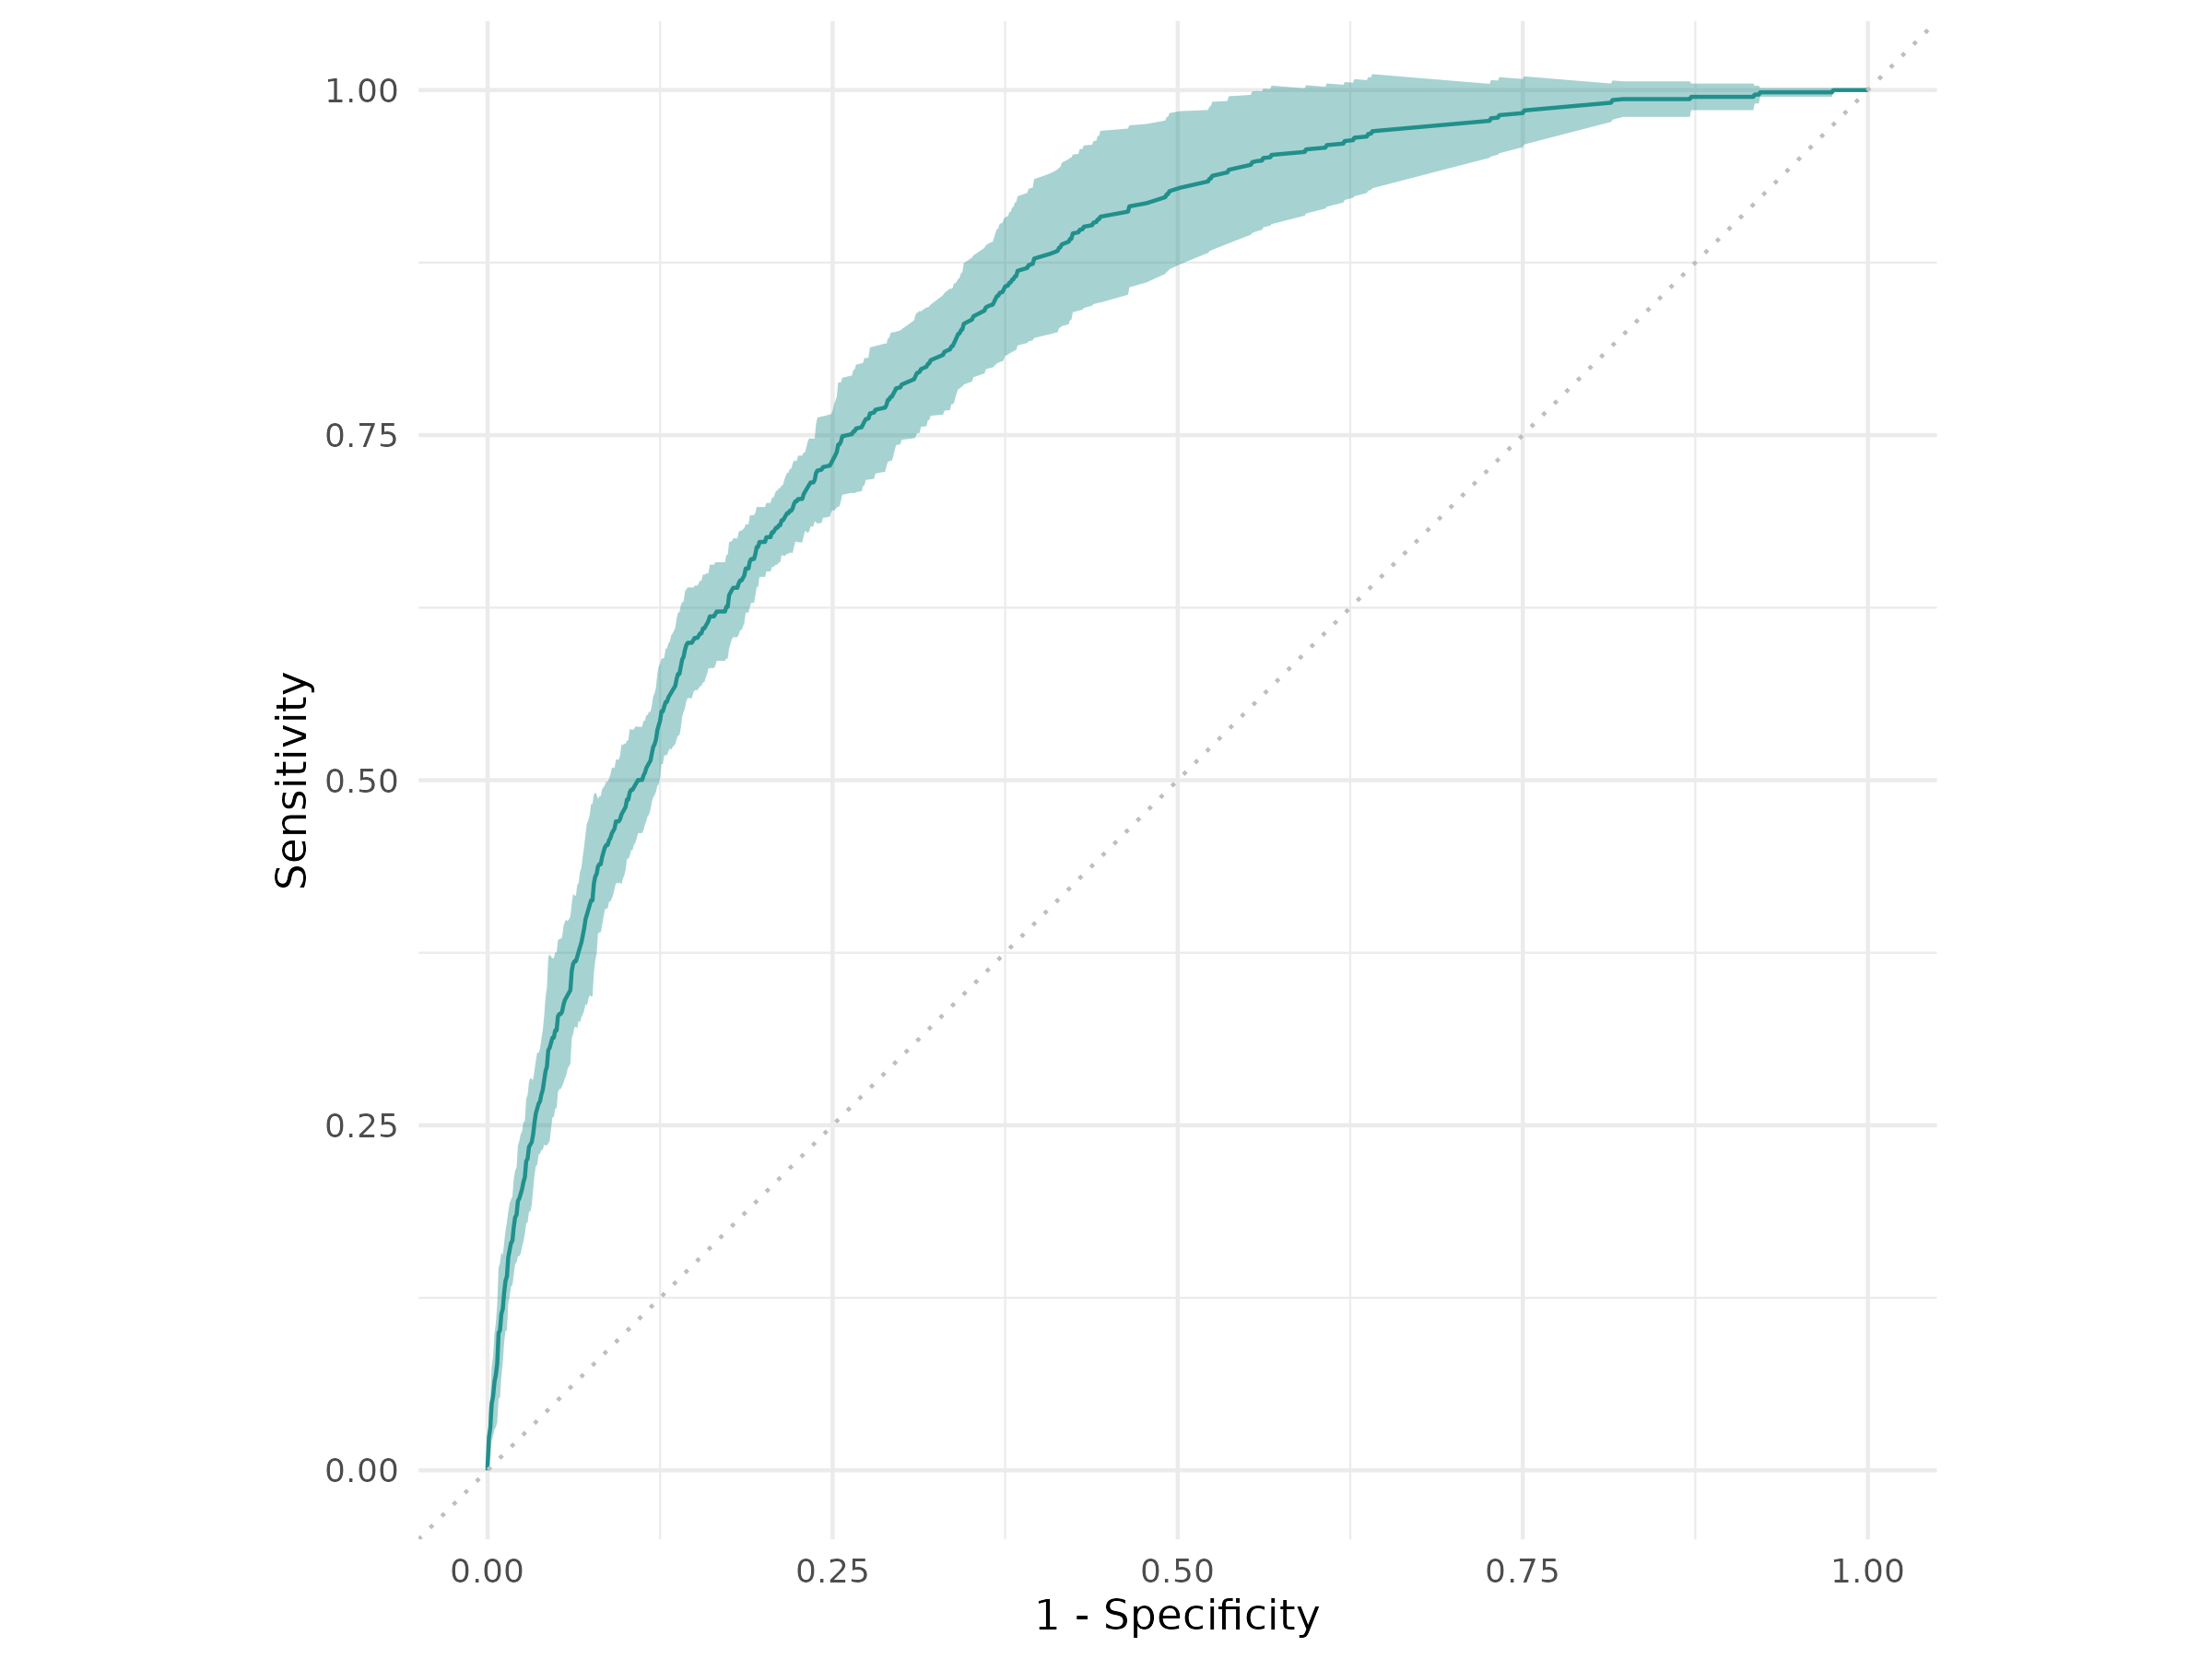
\includegraphics[width=0.4\textwidth]{figures/roc.png}
    \caption{ROC curve for the multimodal neural network evaluated using 5-fold cross-validation.}
    \label{fig:roc-curve}
\end{figure}

\section{Runtime evaluation}\label{sec:benchmarks}

The primary contribution of this work is that it provides a high-level interface to DL in \rlang{} and the main computational tasks are handled by the \torch{} backend.
The main component influencing the runtime performance of this package is therefore \torch{} and not \mlrttorch{}.
Nonetheless, the training speed is an important consideration for users when deciding whether to use the package, especially for DL models, which are notoriously expensive to train.
Furthermore, it is important to ensure that \mlrttorch{} does not add a significant framework overhead over a pure \torch{} implementation.
In this section, we present runtime benchmarks that compare a simple training loop using \mlrttorch{} with an equivalent implementation in pure \torch{} and \pytorch{}.
We include \pytorch{} in the evaluation scenario, because it can, due to its popularity and heavy industry investment, be reasonably considered a best-case scenario for the runtime performance of a DL framework.
Despite \torch{} and \pytorch{} being built upon the same \libtorch{} \cpp{} library, there is still a considerable engineering effort in the \pytorch{} "frontend" to make it run as fast as it does.

\subsection{Setup}
One main reason for the success of DL is the use of GPUs for their training, but small neural networks, for example for tabular data, can also be trained on CPUs.
We therefore evaluate the runtime performance on both hardware backends.
We also vary various aspects of the training setup, where the main computational steps are
\begin{itemize}
    \item the forward pass of the neural network, i.e., computing predictions for a given feature vector, as well as the loss calculation,
    \item computing the gradients of the loss function w.r.t. the network's parameters,
    \item performing the optimization step to update the network weights.
\end{itemize}

We train a simple MLP with ReLU activation, different numbers of layers, and latent dimensions on a synthetically generated regression dataset.
Note that the number of floating point operations (FLOPs) scales linearly with the number of layers, but quadratically with the latent dimension.
Moreover, increasing the number of layers causes the creation of more intermediate tensors that are managed by \rlang{} and have to eventually be cleaned up by the \rlang{} garbage collector.

We also use two optimizers: a simple SGD and the more computationally intensive (but realistic) AdamW.
In order to narrow the performance gap between \torch{} and \pytorch{}, we have contributed various improvements to \torch{}, most notably the addition of "ignite" optimizers in \torch{} version 0.14.0.
Instead of implementing the optimization loop in \rlang{}, they wrap the \cpp{} implementation of the optimizers provided in \libtorch{}.

The training runs for a total of 20 epochs on batches of size 32 from a synthetically generated regression dataset with 2000 observations and 1000 features.
Note that we do not vary the number of features because it only influences the computation in the first layer.
We perform a warm-up phase of four epochs to mitigate the impact of constant overheads on timing measurements, ensuring that our reported runtimes more accurately reflect realistic, long-duration training scenarios.
Every experiment is repeated 10 times, and the number of threads for the CPU measurements was set to 1.
The exact computational details are presented in \Cref{app:comp-details}.

\subsection{Results}

We focus on the results for the ignite optimizers, as they are considerably faster than their corresponding \rlang{} implementation and are therefore used in \mlrttorch{}.
The difference between the two versions is especially prevalent for the more expensive AdamW optimizer, where, on the GPU, the relative overhead for a latent size of 1000 ranges from around 1.6 for 0 latent layers to 3.6 for 16 layers.
For the same scenario using SGD, the overhead is only around 1.1.
Usually, however, more complex optimizers like AdamW are used to train neural networks.

\Cref{fig:optimizer-benchmark} displays the absolute time per batch and \Cref{fig:optimizer-benchmark-relative} shows relative results.


\begin{figure}[h]
    \centering
    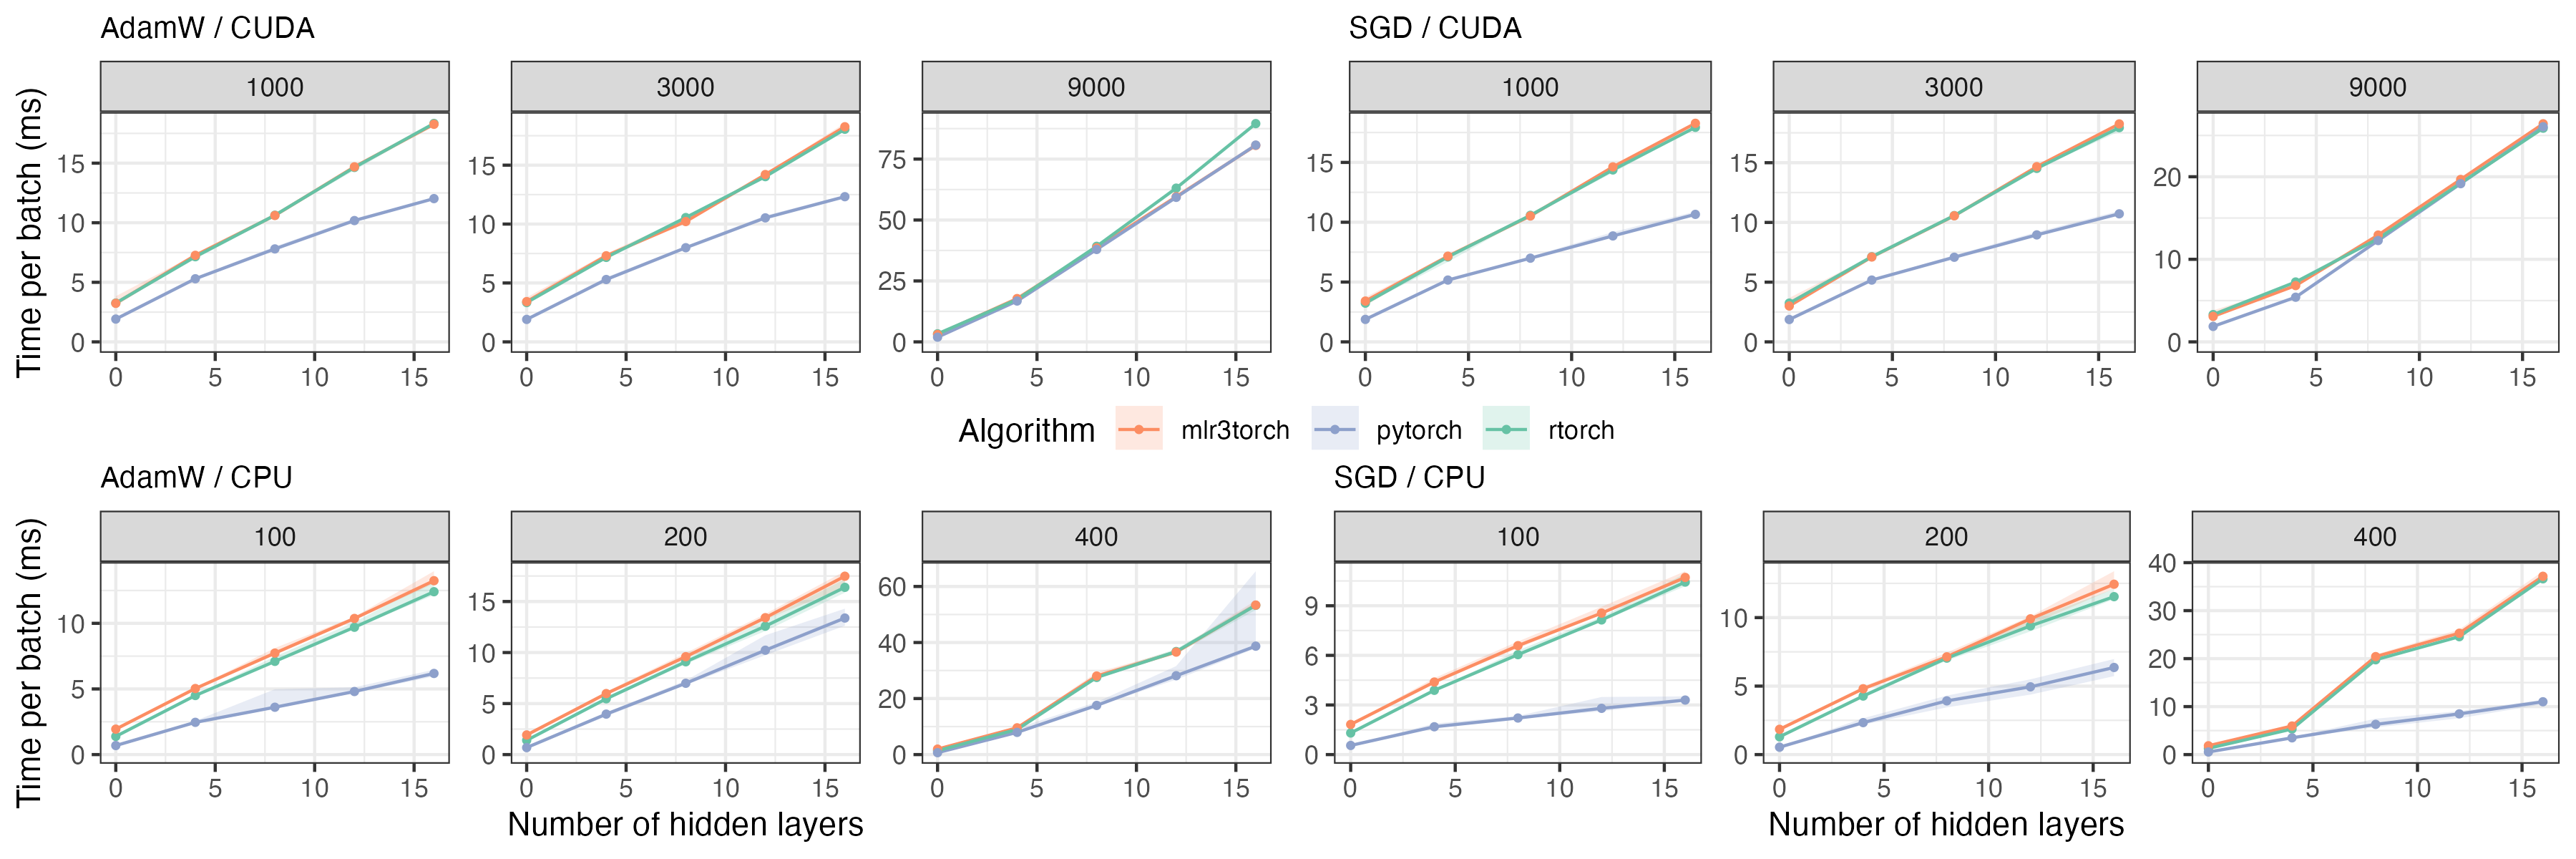
\includegraphics[width=\textwidth]{figures/plot_benchmark.png}
    \caption{Runtime results for AdamW (left) and SGD (right) for GPU (top) and CPU (bottom). The facets correspond to different latent dimensions. The number of hidden layers is $0, 4, 8, 12, 16$.
    The lines represent the median and the shaded area is defined by the upper and lower 10\% quantile of the 10 repetitions.
}
    \label{fig:optimizer-benchmark}
\end{figure}

\begin{figure}[h]
    \centering
    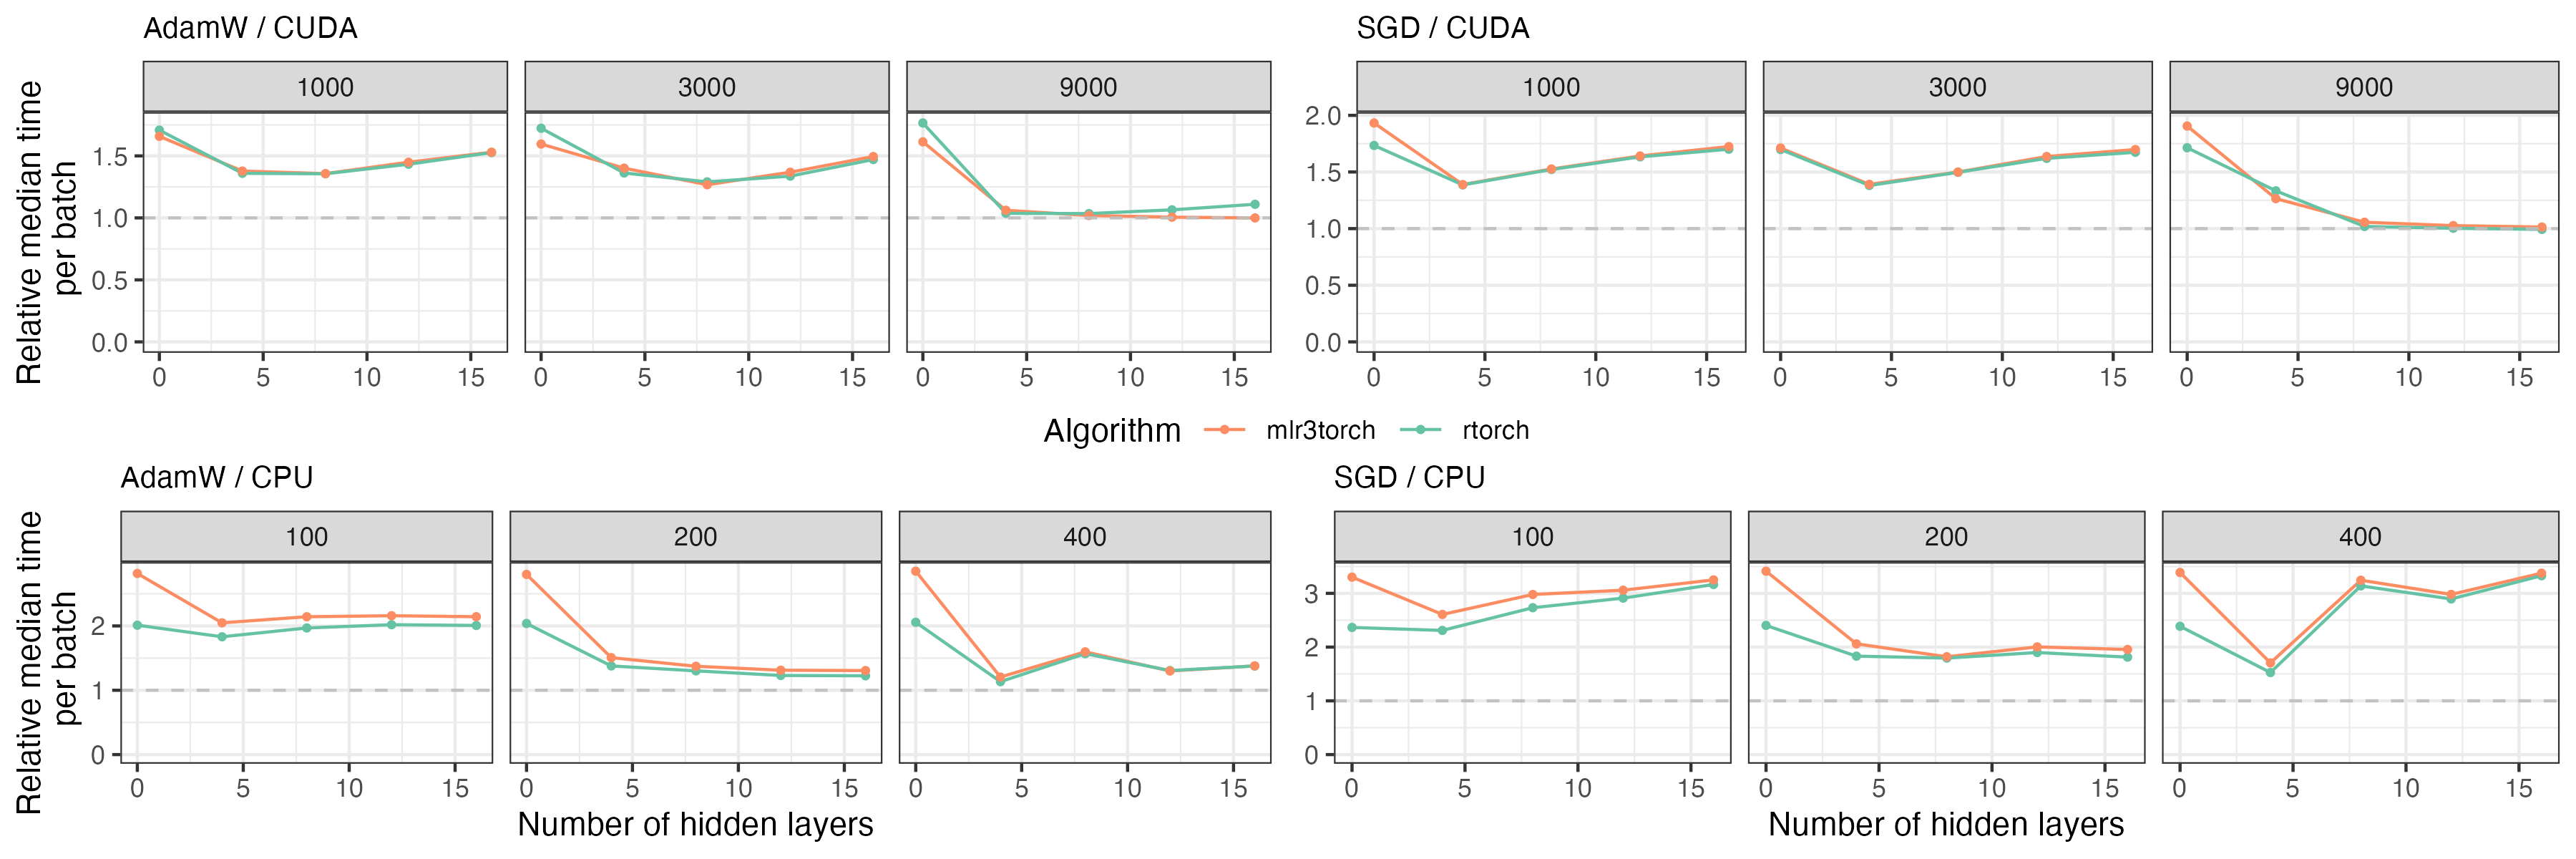
\includegraphics[width=\textwidth]{figures/plot_benchmark_relative.png}
    \caption{Median runtime of \mlrttorch{}  and \torch{} relative to \pytorch{}.}
    \label{fig:optimizer-benchmark-relative}
\end{figure}

% 1. torch in R zu verwenden gibt einem sehr schnelles DL.
% 2. wie groß und substrantiell ist OH von mlr3torch im vgl zu rtoch und zu pytorch
% hängt er von besponderen aspekten wie größe des NNs und device, (aber auch n und p? das verändern wir leider nicht....)
% wie viel schneller ist GPU vs CPU?


In all experiments, the results of \torch{} and \mlrttorch{} are relatively similar.
Only when the neural network is relatively small is the relative overhead more noticeable, which is expected.

% CUDA
When training on the GPU, the relative overhead of \torch{} w.r.t. \pytorch{} diminishes when increasing the latent dimension.
This is not always the case when increasing the number of hidden layers.
For example, for latent dimensions 1000 and 3000, the absolute overhead also increases with more layers, but when the network becomes very large, all three implementations are very similar.
Surprisingly, \mlrttorch{} is slightly faster than \torch{} for the AdamW optimizer when there are many layers and the number of latent dimensions is 9000, but this is likely an artifact explained by some internal mechanism of \torch{} or \libtorch{}.

% CPU
On the CPU, both the relative and absolute overhead of the \rlang{} implementations is larger for SGD than it is for the more compute and memory-intensive AdamW optimizer.
Also, the relative overhead for the AdamW optimizer decreases with an increase in the number of hidden layers, which is not the case for the SGD optimizer.
This shows that there is some optimization potential to be explored for the latter.

The benchmark also demonstrates the runtime advantage of the GPU over the CPU.
When changing the latent dimension from 100 to 1000, this causes -- due to the quadratic scaling -- a 100-fold increase in the number of FLOPs.
However, the time per batch is relatively similar, due to the different hardware backends, indicating a speed-up of around two orders of magnitude when using a GPU.

Overall, the runtime performance of \mlrttorch{} and \torch{} can be considered reasonable, especially when focusing on the arguably most realistic case of training a neural network on the GPU using the AdamW optimizer.

\section{Conclusion}\label{sec:conclusion}

In this work we introduced \pkg{mlr3torch} --- an extensive DL framework in \rlang{} that integrates with the \mlrt{} ecosystem.
This enables seamless access to operations like resampling, benchmarking, and hyperparameter tuning.

The package offers a unified interface for defining, training, and evaluating neural networks, with support for both tabular data and generic tensors in supervised classification and regression tasks.
Neural network architectures are available in different levels of control: predefined architectures are readily available, \torch{} modules can be easily converted to \mlrttorch{} learners, and custom architectures can be defined as graphs.
Enabled by the lazy tensor data type and the integration with \mlrtpipelines{}, the whole modeling workflow (including preprocessing, data augmentation, and the definition of the neural network itself) can be represented as a single graph.

A key strength of \pkg{mlr3torch} is its extensibility and flexibility, be it in defining architectures, customizing the training, e.g., via the provided callback mechanism, or the possibility to extend the package.
We demonstrated the package's reasonable through three practical use cases. First, we showed how to perform neural architecture search on a tabular regression problem.
Second, we fine-tuned a pre-trained ResNet-18 model to a binary image classification task.
Finally, we showcased the framework's ability to define architectures with multiple inputs for a multimodal task that contained both tabular data and images.

Our runtime benchmarks demonstrate reasonable framework overhead of \mlrttorch{} compared to a pure \torch{} implementation.

Future development will focus on extending support to other learning tasks such as survival analysis, implementing additional architectures, further improving runtime performance, and extending the support to other modalities like natural language.

%\input{6-conclusion}

\section*{Acknowledgements}

Sebastian Fischer is supported by the Deutsche Forschungsgemeinschaft (DFG, German Research Foundation) – 460135501 (NFDI project MaRDI).

\bibliography{refs}

\begin{appendix}

\newpage
\section{Reproducibility}\label{app:comp-details}

% Computational environment
For reproducibility purposes, we provide two Docker containers -- one for GPU (CUDA) and one for CPU -- that can be downloaded from here: \url{https://hub.docker.com/repository/docker/sebffischer/mlr3torch-jss/general}.
Note that \torch{} comes with its own BLAS implementation, so \rlang{} being installed with the default BLAS does not hurt performance.

% Code for reproducibiluty
The code to reproduce all results from this article, as well as instructions on how to do so, is provided in the ./paper subdirectory of the software's GitHub repository: \url{https://github.com/mlr-org/mlr3torch}.

% Hardware & OS
All experiments were run on Linux.
Code requiring access to a GPU was run on an NVIDIA HGX A100 with 80 GB VRAM.
The CPU was an Intel(R) Xeon(R) Gold 6336Y CPU @ 2.40GH with 1 TB RAM and 48 physical cores.
The CPU benchmark was run on an Intel(R) Xeon(R) Gold 6226R CPU @ 2.90GHz with 32 physical cores and 12 8GB RAM.

% Non-reproducibilility issues
Due to the combination of parallelism and floating point arithmetic, some CUDA operations are non-deterministic even when setting the seed.
While \libtorch{} offers deterministic, albeit slower, versions for some algorithms, some kernel operations have no deterministic variant at all. This includes the derivative of the max pooling operation used in the ResNet-18 model from~\Cref{sec:finetuning}.
Therefore, the results are not exactly reproducible after the second epoch (because during the first two epochs, only the output head is trained), and performance differences of about 0.2\% can be observed when reproducing the results.
For this reason, we also include a script that contains a simplified version of the code from the paper that is running on the CPU and which is fully reproducible and -- due to the simplification -- runs very quickly.
\end{appendix}


\end{document}
